\documentclass{CMHPhD-SIVD}

\begin{document}
%\begin{frontmatter}  % not sure this is needed for T&F


% Specify the article type or omit as appropriate
%\articletype{ARTICLE TEMPLATE}
% JW - suggest we leave this for the print editor to worry about

\title{
  An eclipse-phase lag drives oscillations in a viral infection model with a general growth function}

\author{
	\name{
		Menghan Chen\textsuperscript{a}
	    %\thanks{CONTACT Menghan Chen Email: cmhmath1210@163.com}
    and Lin Wang\textsuperscript{b}
		and James Watmough\textsuperscript{b}
	    \thanks{CONTACT James Watmough Email: watmough@unb.ca}
	}
	\affil{
		\textsuperscript{a}
	  Department of Mathematics, Shanghai University, Shanghai 200444, China;
	  \textsuperscript{b}
		Department of Mathematics and Statistics, University of New Brunswick, Fredericton, E3B 5A3, Canada
	}
}

\maketitle

\begin{abstract} %150 words (need to shrink)
	Stable and sustained oscillatory patterns are often found in viral infections such as hepatitis B virus, HIV and even SARS-CoV-2. As we know, it is closer to the actual biological significance to consider the survival rate of infected cells from activation to infectivity, and the reduction in the number of virus due to infection of host cells. However, this process is neglected in some theoretical models, but which is regarded as a key issue in our study. Therefore, we developed a new model based on the Jenner et al.\ model to explore the role of time delay and important parameters on the rich dynamics of the system. In this paper, the basic reproduction number $R_0$ of the virus-infected system is derived. The stability of the time delay to the infection-free equilibrium, and the stability and the Hopf bifurcation analysis of the infection-present equilibrium are given. Our results suggest that the stability of the  infection-free equilibrium also changes under different $R_0$ conditions. In addition, the change of the time delay can induce the oscillatory behavior of the system at the infection-present equilibrium, and then generate the Hopf bifurcation. Finally, some numerical simulations such as one-parameter and two-parameter bifurcation diagrams of the delay bifurcation values to parameters are carried out on the delay and important parameters.
\end{abstract}


\begin{keywords}
Viral dynamic; Time delay; Stability; Hopf bifurcation; Periodic oscillations
%% keywords here, in the form: keyword \sep keyword
\end{keywords}

%\end{frontmatter}

\linenumbers

\section{Introduction}
Viral dynamic models have received increased and widespread attention since the onset of the CoViD-19 pandemic \cite{zu2021investigating,wang2021effects,tang2022controlling,qian2020modelling}.
This renewed interest builds on earlier mathematical models describing the process of infection in vivo \cite{smith2003virus,wang2006mathematical,li2012joint,mojaver2015mathematical,pan2019rich}.
Mathematical models can include key features of the infection process and their analysis can provide guidance for the development of antiviral drugs. It is precisely because models of in-host infection dynamics have important biological significance for the spread and control of infectious diseases that most scholars have carried out dynamic analyses of such models \cite{li2010global,li2010impact,shu2014sustained}. In addition, many scholars have proposed that the inherent intracellular time delay and sudden changes in various rates in the host cell have a crucial impact on the virus dynamics \cite{culshaw2000delay,huang2010lyapunov,vargas2012stability,shu2015delay,pertsev2019stochastic,lu2021mathematical}.

All in-host mathematical models include two core components: virus entry into host cells, and virus release from host cells. The classic model including host cells, infected cells, and viruses was first formulated by Neumann et al.\ \cite{neumann1998hepatitis} and used in the study of antiviral therapy. Wang et al.\ \cite{wang2006mathematical} and De Leenheer and Smith \cite{smith2003virus} considered the logistic growth term in their viral kinetic models, but did not take into account the time delay between virus entry into target cells and subsequent virus production from newly infected cells, known as the eclipse period. Their results indicate that Hopf bifurcation induced sustained oscillations appear when the growth rate increases.
Culshaw \cite{culshaw2000delay} and Wang et al.\ \cite{wang2009oscillatory} considered not only the logistic growth term but also the eclipse time delay and showed that the equilibrium could undergo Hopf bifurcations as the time delay increased. Based on these studies, to gain insight into the combined effects of target cell dynamics and delay on viral dynamics, Li et al.\ performed a two-parameter bifurcation analysis \cite{li2012joint}.

In response to the rapid spread of CoViD-19, Jenner et al.\ formulated an SIVD model that includes two mechanisms thought important to SARS-CoV-2 dynamics: the eclipse time delay and the impact of dead cells on the host cell dynamics\cite{jenner2021covid}.
The authors provide a computational study of the model, but do not provide a corresponding explanation for the complex dynamics resulting from changing the time delay.   The main objective of our present paper is to provide a theoretical analysis of a generalization of the time-delayed SIVD and to catalog some of the complex dynamics induced by the delay.

The delay differential equation of Jenner et al.\ is shown as follows:
\begin{subequations}\label{SIVD-J}
   \begin{align}
		 \dot{S} &= \lambda\left(1-\frac{S(t)+I(t)+D(t)}{\Smax}\right)S(t)-\beta S(t)V(t),
		 \label{SIVD-SJ}\\[3pt]
		 \dot{I} &= \beta S(t-\tau)V(t-\tau)-d_I I(t),
		 \label{SIVD-IJ}\\[3pt]
         \dot{V} &= pI(t)-d_V V(t),
		 \label{SIVD-VJ}\\[3pt]
		 \dot{D} &= d_I I(t)-d_D D(t).
		 \label{SIVD-DJ}
   \end{align}
\end{subequations}

In the model, $S(t)$, $I(t)$, $V(t)$ and $D(t)$ represent susceptible cells, infected cells, free virus and dead cells, respectively. The parameters $d_I$, $d_V$ and $d_D$ represent the natural mortality of $I(t)$, $V(t)$ and $D(t)$ compartments, respectively. Here, they argue that cell proliferation induced by mitosis follows a logistic growth law. Mitotic proliferation of susceptible cells is represented by the logistic term $\lambda\left(1-\frac{S(t)+I(t)+D(t)}{\Smax}\right)S(t)$.  The new infection transmission term is denoted by $\beta S(t)V(t)$, where $\beta$ is the infection rate constant. Infected cells can produce free viral particles, where $p$ is the production rate. Finally, the infected cells are cleared and turned into dead cells, which is represented as the first term $d_I I$ in the variable $D(t)$.


Jenner et al.\ used a stepwise approach to parameter estimation in the context of CoViD-19, and the resulting model dynamics were well consistent with these early infection data. In addition, the results showed a rebound in lung epithelial tissue as viral load and infected cells decreased. Although the work of Jenner et al.\ is relatively novel, the model has not been comprehensively considered. In our paper, we propose a more realistic model based on the model of Jenner et al., which is embodied as follows:
\begin{subequations}\label{SIVD}
   \begin{align}
		 \dot{S}(t) &= f(S(t), I(t), D(t))-\beta_1 S(t)V(t),
		 \label{SIVD-S}\\[3pt]
		 \dot{I}(t) &= \beta_1 e^{-\delta \tau}S(t-\tau)V(t-\tau)-d_I I(t),
		 \label{SIVD-I}\\[3pt]
				 \dot{V}(t) &= pI(t)-\beta_2 S(t)V(t)-d_V V(t),
		 \label{SIVD-V}\\[3pt]
		 \dot{D}(t) &= d_I I(t)-d_D D(t).
		 \label{SIVD-D}
   \end{align}
\end{subequations}
%\lambda_S\left(1-\frac{S(t)+I(t)+D(t)}{\Smax}\right)S(t), \beta_1 S(t)V(t)

Here, the net growth of susceptible cells is denoted by a general function $f$ satisfying the following conditions:

\hypothesis{1}
  $f\in C^1(\mathbb{R}_+^3)$,
	there exists $\Smax>0$ such that $f(0,I,D)=f(\Smax,0,0)=0$,
	$f(S,0,0)(S-\Smax)<0$ for $S\neq \Smax$ and $S>0$, and
	$f(S,I,D) < f(S,0,0)$, $\frac{\partial f}{\partial S}(0,0,0)>0$.

Furthermore, it is well known that infected cells do not immediately become infectious, but undergo an eclipse phase. It is assumed that infected cells infected at time $t-\tau$ become infectious at time $t$. The probability of survival of infected cells during the delay period from $t-\tau$ to $t$ is also of particular importance in many infection kinetic studies \cite{xu2011global,song2010properties,bera2015delay,sazonov2020viral}. Therefore, we consider this phenomenon based on the model of Jenner et al.\ and express it in terms of $e^{-\delta \tau}$. Another crucial situation to note is that when the virus infects the host cell, the free virus is also reduced, here denoted $\beta_2 S(t)V(t)$, and the virus enters the host cell at the rate of $\beta_2$. The schematic diagram of this host-pathogen interaction is shown in \fig{Fig.1}.

\begin{figure}[h!]
\centering
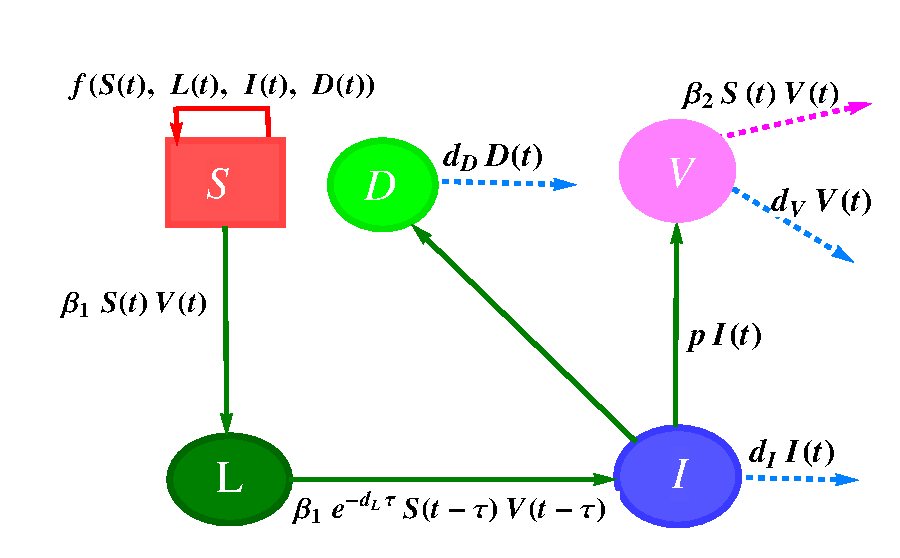
\includegraphics[height=0.350\textheight,width=0.7\textwidth]{s.eps}
\vspace{3mm}
\caption{Schematic diagram of this host-pathogen interaction.}
\label{Fig.1}
\end{figure}

In general, dynamic phenomena such as stability of equilibrium points and sustained oscillations caused by changes in the time delay are an interesting topic in biological systems. Compared with existing research in related fields, the novelty of our paper lies in the following aspects. First, in this paper, based on the Jenner et al.\ model, we consider the possibility of the survival of infected cells from $t-\tau$ to $t$.  Crucially, virus reduction due to virus infection of host cells is considered in our model. Secondly, in this paper, the stability and Hopf bifurcations with time-delay and no-delay are studied theoretically and numerically at infection-free and infection-present equilibriums. In addition, the results of the numerical simulations are consistent with the theoretical predictions. Third, this study can be seen as a complement to the work of Jenner et al., and clearly shows that time delay is important for the dynamic mechanism of viral infection models.

Our main purpose in this paper is to analyze the complex dynamics in the time-delay differential equations (\ref{SIVD}) from a theoretical perspective and to provide clues to experimental observations of virus dynamics. Our paper mainly consists of the following aspects. First, the positivity and uniform boundedness of solutions are established. Next, in Section \ref{sec3.1}, the basic reproduction number is derived. In Section \ref{sec3.2}, the stability analysis of the infection-free equilibrium point $E_0$ is given by the corresponding characteristic equation and normal form. In Section \ref{3.3}, the stability and the Hopf bifurcation of the  infection-present equilibrium point $E_1$ are discussed. Specifically, the stability at $\tau=0$ and the Hopf bifurcation at $\tau>0$ are analyzed. In Section \ref{sec4}, some numerical simulations for supporting the theoretical analysis are done. Finally, conclusions and summaries are presented in Section \ref{sec5}.




\section{Preliminaries}
To analyze the dynamics of System (\ref{SIVD}), we need to consider a reasonable phase space and range. For $\tau>0$, let $\mathscr{C}=\mathcal{C}([-\tau,0],\mathbb{R})$, the Banach space of continuous functions on $[-\tau,0]$, with norm $\|\phi\|=\rm sup_{-\tau\leq\theta\leq0}|\phi(\theta)|$ for all $\phi\in\mathscr{C}$. The nonnegative cone of $\mathscr{C}$ is denoted as $\mathscr{C}^+=\mathcal{C}([-\tau,0],\mathbb{R}_+)$. Let $X=\mathcal{C}([-\tau,0],\mathbb{R}^4_+)$. Given $u\in\mathcal{C}([-\tau,\infty),\mathbb{R})$ and time t, define $u_t\in\mathscr{C}$ by $u_t(\theta) = u(t+\theta)$, $\theta\in[-\tau,0]$. 
We are interested in solutions to System (\ref{SIVD}) with nonnegative initial conditions:
\begin{align*}
(S_0, I_0, V_0, D_0) \in X.
\end{align*}
\jwmargin{$X$ now has $I$ and $D$ as functions.  Check consistency everywhere.
}

\begin{lemma}\label{2.1}
Suppose $h$ satisfies \hypothesis{1}
and let $g:x\to s(\Smax-x)$ with $s=\max\left\{\frac{h(x,0,0)}{\Smax-x}\right\}$.
Then
	\begin{enumerate}[(i)]
		\item $h(x,y,z)<h(x, 0, 0)\leq g(x)$ for $x\in\mathbb{R}_3^+$; and
		\item every solution to the differential inequality $x'\leq g(x)$ with $x(0)\leq \Smax$ satifies $x(t)\leq \Smax$.
	\end{enumerate}
\end{lemma}

 %Consider System (\ref{SIVD}) with any initial condition ($S(0)$, $I_0$,$V(0)$,$D(0)$)$\in \mathbb{R}_+^4\times \mathcal{C}^+\times \mathcal{C}^+$, where $I(\theta)=I_0$, $\theta\in(-\tau,0)$.

\begin{proposition}  Under the above initial conditions, all solutions of System (\ref{SIVD}) are nonnegative and ultimately bounded. 
Let $\Gamma$ be subset of all points $(S, I, V, D) \in X$ satisfying the bounds

\begin{enumerate}[(i)]
	\item $0<\|S\|\leq \Smax$
	\item $S(-\tau)+I(0)\leq\frac{s}{\tilde{\mu}} \Smax$
	\item $\|V\|\leq\frac{ p s}{d_V\tilde{\mu}} \Smax$
	\item $D(0)\leq\frac{d_I s}{d_D\tilde{\mu}} \Smax$
\end{enumerate}
with $\tilde{\mu}=\min\{s,d_I\}>0$ is positive invariant and attracting.
\end{proposition}
\jwmargin{jw check $I$ and $D$ against definition of $X$. Do they need (0)'s?}


\begin{proof} For any given $\phi\in X$, let us define
	$\chi:X\to\mathbb{R}^4$ by
\begin{equation}\label{38}
     \chi(\phi)=
     \begin{pmatrix}
			 \chi_1(\phi) \\ \chi_2(\phi) \\ \chi_3(\phi) \\ \chi_4(\phi)
		 \end{pmatrix}=
     \begin{pmatrix}
     f(\phi_1(0), \phi_2(0), \phi_4(0))-\beta_1 \phi_1(0)\phi_3(0)\\
      \beta_1 e^{-\delta \tau} \phi_1(-\tau) \phi_3(-\tau) -d_I \phi_2(0)  \\
     p\phi_2(0)-\beta_2 \phi_1(0) \phi_3(0)-d_V \phi_3(0)\\
     d_I \phi_2(0)-d_D \phi_4(0)
     \end{pmatrix}.
\end{equation}
$\chi(\phi)$ is continuous for $\phi\in X$ and Lipschitz in $\phi$ on each compact set of $X$. Since $\chi_i(\phi)\geq0$ whenever $\phi \in X$ with $\phi_i(0) = 0$, it follows that the solution $(S(t), I(t),V(t),D(t))^\top$ is nonnegative (See Theorem 5.2.1 in \cite{smith1995monotone} and \cite{guo2018global}).


%From the first equation (\ref{SIVD-S}), we can obtain

%\begin{eqnarray*}
%S(t)=S(0)e^{\int_0^t\left[\lambda_S\left(1-\frac{S(\theta)+I(\theta)+D(\theta)}{\Smax}\right)-\beta_1 V(\theta)\right]d\theta}>0
%\end{eqnarray*}

%Next, we prove that $V(t)$ is positive for all $t\geq0$. Assuming the contrary, and letting $t_1>0$ be the first time such that $V(t_1)$=0 and $V'(t_1)<0$, by the third equation (\ref{SIVD-V}), we obtain $V'(t_1)=pI(t_1)$. Solving the $I(t)$ in the second equation (\ref{SIVD-V}), we obtain
%\begin{eqnarray*}
%I(t_1)=e^{-d_I t}\left(I(0)+\int_0^{t_1} \beta_1 e^{-\delta \tau}S(\theta-\tau)V(\theta-\tau)e^{d_I \theta}d\theta\right)>0
%\end{eqnarray*}

%It follow that the $V'(t_1)>0$, this contradicts $V'(t_1)<0$. Therefore, $V(t)$ is positive, then
%\begin{eqnarray*}
%I(t)=e^{-d_I t}\left(I(0)+\int_0^t \beta_1 e^{-\delta \tau}S(\theta-\tau)V(\theta-\tau)e^{d_I \theta}d\theta\right)>0
%\end{eqnarray*}



%From the forth equation (\ref{SIVD-D}), we can obtain
%\begin{eqnarray*}
%D(t)=e^{-d_D t}\left(D(0)+\int_0^t d_I I(\theta) e^{d_D \theta}d\theta\right)>0
%\end{eqnarray*}
%
%As can be seen from the above expression, we conclude that all solutions in the model are positive for $t > 0$.





Next, we show that all solutions of System (\ref{SIVD}) with nonnegative initial conditions are uniformly bounded.
	Suppose $(S, I,  V,  D)$ is a solution to \eqn{SIVD} with nonnegative initial conditions.  Then by the above we know $(S_t,I_t,V_t,D_t)\in X$ for all $t >0$.
	From \eqn{SIVD-S}, we obtain
\begin{align*}
S'(t)\leq f(S(t), I(t), D(t)),   \qquad t\geq0,
\end{align*}
	and by Lemma \ref{2.1} $(ii)$, if $0<S(0)\leq \Smax$, then $0< S(t)\leq \Smax$.
	Hence, $S$ is uniformly bounded and $0 < \|S(t_0)\| < \Smax$ implies $0 < \|S(t)\| < \Smax$ for all $t>t_0$, establishing the first part of the positive invariance of $\Gamma$.
Next, adding Equations (\ref{SIVD-S}) and (\ref{SIVD-I}) and applying Lemma \ref{2.1} $(ii)$, we obtain
\begin{align}\label{37}
\left(S(t-\tau)+I(t)\right)'&=f(S(t-\tau), I(t-\tau), D(t-\tau))\nonumber \\
&+\beta_1 S(t-\tau)V(t-\tau)(e^{-\delta\tau}-1)-d_I I(t)\nonumber \\
&
\leq s \Smax-s S(t-\tau)+\beta_1 S(t-\tau)V(t-\tau)(e^{-\delta\tau}-1)-d_I I(t)\nonumber \\
&
\leq s \Smax-\tilde{\mu}\left(S(t-\tau)+I(t)\right)
\end{align}
where $\tilde{\mu}=\min\{s,d_I\}$. 
Any solution to this differential inequality with initial values $S(-\tau)$ and $I(0)$ satisfies
\begin{align*}
S(t-\tau)+I(t)\leq e^{-\tilde{\mu}t}(S(-\tau)+I(0))+\frac{s \Smax}{\tilde{\mu}}\left(1-e^{-\tilde{\mu}t}\right),
\end{align*}

This establishes the second component of the positive invariance of $\Gamma$: namely, that $0 < S_t(-\tau) + I(t) < \frac{s}{\tilde{\mu}}\Smax$ for all $t>t_0$ provided $0 < S_{t_0}(-\tau) + I(t_0) < \frac{s}{\tilde{\mu}}\Smax$.




%Then,
%\begin{align*}
%\lim_{t\rightarrow \infty} \sup (S(t)+I(t+\tau))\leq \frac{\lambda_S \Smax}{\tilde{\mu}}.
%\end{align*}



\eqn{SIVD-V} implies
\begin{eqnarray}\label{39}
V'(t)\leq \frac{ps \Smax}{\tilde{\mu}}-d_V V(t)
\end{eqnarray}

From \eqn{39}, we can obtain
\begin{align*}
V(t)\leq e^{-d_V t}V(0)+\frac{p s \Smax}{d_V\tilde{\mu}}\left(1-e^{-d_V t}\right),
\end{align*}

Hence, $V(t)$ is uniformly bounded and, if $\|V_{t_0}\| \leq \dfrac{ p s \Smax}{d_V\tilde{\mu}}$ at some time ${t_0}$,  then $\|V_t\| \leq \dfrac{ p s \Smax}{d_V\tilde{\mu}}$ for all $t>t_0$, establishing the third component of the positive invariance of $\Gamma$.

%\begin{eqnarray*}
%V'(t)\leq\frac{ p \lambda_S \Smax}{\tilde{\mu}}-d_V V(t)
%\end{eqnarray*}
%and lim sup$_{t\rightarrow\infty}V(t)\leq\frac{ p \lambda_S \Smax}{d_V\tilde{\mu}}$.


Finally, \eqn{SIVD-D} implies
\begin{eqnarray}\label{40}
D'(t)\leq  \dfrac{d_I s \Smax}{\tilde{\mu}}-d_D D(t)
\end{eqnarray}
From \eqn{40}, we obtain
\begin{align*}
D(t)\leq e^{-d_D t}D(0)+\dfrac{d_I s \Smax}{d_D\tilde{\mu}}\left(1-e^{-d_D t}\right),
\end{align*}

Hence, $D(t)$ is uniformly bounded and $D(t_0)\leq \dfrac{ d_I s \Smax}{d_D\tilde{\mu}}$ implies $D(t)\leq \frac{d_I s \Smax}{d_D\tilde{\mu}}$ for all $t>t_0$. This establishes the final component of the positive invariance of $\Gamma$.


%Therefore, the system (\ref{SIVD}) has positive invariant sets
%\begin{eqnarray*}
%\Upsilon=\left\{(S(0),I_0,V(0),D(0))\in\mathbb{R}_+^4\times \mathcal{C}^+\times \mathcal{C}^+:0\leq \|S\|\leq \Smax,S(-\tau)+I(0)\leq\frac{\lambda_S \Smax}{\tilde{\mu}}, 0\leq \|V\|\leq\frac{ p \lambda_S \Smax}{d_V\tilde{\mu}}, 0\leq \|D\|\leq\frac{d_I \lambda_S \Smax}{d_D\tilde{\mu}}\right\}
%\end{eqnarray*}
\end{proof}

\section{Existence and stability of equilibria}

\subsection{Existence, uniqueness, and $R_0$}\label{sec3.1}
System (\ref{SIVD}) has a two infection-free equilibrium: $(0,0,0,0)$ and $E_0=(\Smax,0,0,0)$.
The characteristic equation associated with the linearization of System (\ref{SIVD}) about $E_0$ is
\begin{equation}\label{4}
	\left(\lambda-\frac{\partial f}{\partial S} (\Smax, 0, 0)\right)(\lambda+d_D)\left[\lambda^2+A_1\lambda+A_2-A_3e^{-\lambda\tau}\right]=0,
\end{equation}
%\end{footnotesize}
where
\begin{align*}
&A_1=(d_I+d_V+\beta_2 \Smax),\\
&A_2=(\beta_2 \Smax+d_V)d_I,\\
&A_3=p\beta_1 \Smax e^{-\delta\tau}.
\end{align*}

%To formulate the basic reproduction number, partition the lower right block of $J$ into two parts as follows:
%
%\begin{equation}\label{SIVD-FVsplit}
% J= F-V =
%\begin{pmatrix}
%  0 & 0  & 0\\
%	p & 0  & 0 \\
%  0 & 0  & 0
%  \end{pmatrix}
%	-
%\begin{pmatrix}
%  d_{I}   & -\beta_1 e^{-\delta\tau}\Smax   & 0 \\
%   0      &  \beta_2 \Smax+d_{V}              & 0\\
%   -d_{I} & 0  & d_{D}
%  \end{pmatrix}
%\end{equation}
%
%In this partitioning we view the virus as progressing from a free stage to an in-cell stage at rate $\beta_1$, and free virus being produced by the in-cell stage.  The basic reproduction number is $\rho(FV^{-1})$.


%We let $\lambda=0$.
Therefore, the basic reproduction number is
\begin{equation}\label{SIVD-Ro}
   R_0=\frac{\Smax p \beta_1 e^{-\delta \tau}}{d_{I}(d_{V}+\Smax \beta_2)},
\end{equation}
\jwinline{Ro is not defined via the characteristic equation.  Better to introduce it where first used and motivate it epidemiologically (see comment on next page).  Since the characteristic equation is not used for anything else here, suggest moving it to where it is used (local stability of R0=1 case) and keeping this section strictly about existence.}


An infection-present equilibrium has the form $E_1 = (S_1^*,I_1^*,V_1^*,D_1^*)$with $S_1^*$, $I_1^*$, $V_1^*$, and $D_1^*$ satisfing the following conditions and $I_1^*$ nonzero: 
\begin{subequations}
\begin{align}
&f(S_1^*, I_1^*, D_1^*)=\beta_1 S_1^* V_1^*, \label{S1}\\
&I_1^*=\frac{e^{-\delta\tau}}{d_I}f(S_1^*, I_1^*, D_1^*), \label{I1}\\
&V_1^*=\frac{p e^{-\delta\tau}}{d_I(\beta_2 S_1^*+d_V)}f(S_1^*, I_1^*, D_1^*),\label{V1}\\
&D_1^*=\frac{d_I}{d_D}I_1^*. \label{D1}%\frac{e^{-\delta\tau}}{d_D}f(S_1^*, I_1^*, D_1^*),
\end{align}
\end{subequations}
\jwinline{Might be wise to drop the subscript 1 to avoid confusion with the $S_t$ notation.  Do we need both the subscript 1 and the superscript *?}

\jwinline{It is convenient to have the main results typeset as theorems or lemmas for easy reference.  I think our lemma here is the existence and uniqueness of $E_1$ for $R_0 > 1$.  Which makes this the best place to introduce Ro.  We can do this nicely with a bit of preamble to the lemma.}

\jwinline{
Substituting the \eqn{V1} into the \eqn{S1} leads to the condition
	$f(S^*, I^*, D^*)\left(1 - R(S^*)\right) = 0$
with $R(S)$ defined as 
\begin{equation}
	R(S) = \frac{\beta_1 p e^{-\delta\tau} S}{d_I(\beta_2 S+d_V)}.
\end{equation}
This dimensionless ratio can be easily interpreted as a fitness of the virus by viewing it as the product of three quantities:  $\frac{p}{d_I}$, the expected virus released per infectious cell; $\frac{\beta_1e^{-\delta\tau}}{\beta_2}$, the infectious cells arising per virus-cell encounter; and $\frac{\beta_2 S}{\beta_2S+d_V}$, the fraction of virus encountering cells.  Hence we introduce the usual notation for the basic reproduction number as 
\begin{equation}
	R_0 = R(\Smax)
	= \frac{\beta_1 p e^{-\delta\tau} \Smax}{d_I(\beta_2 \Smax+d_V)}.
\end{equation}
}

\begin{lemma}
	System (\ref{SIVD}) has a unique infection present equilibria for $R_0>1$.
\end{lemma}
\begin{proof}
Substituting the \eqn{V1} into the \eqn{S1}, then we introduce a function
\begin{align}\label{41}
&f(S, I, D)\left(1-\frac{\beta_1 p e^{-\delta\tau} S}{d_I(\beta_2 S+d_V)}\right)=0.
\end{align}
	\jwmargin{we can use $R(S)$ here and then get to the condition $R(S^*) = 1$ below}
then either $f(S, I, D)=0$, or $\left(1-\frac{\beta_1 p e^{-\delta\tau} S}{d_I(\beta_2 S+d_V)}\right)=0$.  
From $\eqn{S1}$ we see that $f$ can not be zero at an interior equilibrium, hence
$\left(1-\frac{\beta_1 p e^{-\delta\tau} S}{d_I(\beta_2 S+d_V)}\right)=0$. We let
\begin{align*}
&G(S)=1-\frac{\beta_1 p e^{-\delta\tau} S}{d_I(\beta_2 S+d_V)}.
\end{align*}

Clearly, $G(0)=1$, $G(\Smax)=1-\frac{\beta_1 p e^{-\delta\tau} \Smax}{d_I(\beta_2 \Smax+d_V)}=1-R_0$, and $G'(S)=-\frac{\beta_1 p e^{-\delta\tau} d_V}{(d_I(\beta_2 S+d_V))^2}<0$. Therefore, if and only if $R_0>1$, $S_1^*\in[0, \Smax]$ exists and is unique such that $G(S_1^*)=0.$
	\jwmargin{easy to replace $G$ by $R$ here.}

Substituting the equation (\ref{D1}) into the equation (\ref{I1}), we can obtain
\begin{align*}
&d_I I_1^*=e^{-\delta\tau}f(S_1^*, I_1^*, \frac{d_I}{d_D}I_1^*).
\end{align*}

$S_1^*$ is known to be unique. From ($\mathbf{H}_1$) it is known that $f$ decreases with the increase of $I$. Also, the left side of the equation is increase. Therefore, $I_1^*$ is unique. Likewise, $V_1^*$ and $D_1^*$ are also unique. To sum up, if $R_0>1$, the infection equilibrium point $E_1$ exists and is unique.
\end{proof}

%Next we introduce a function
%\begin{align*}
%&G(S)=f(S)-\frac{\beta_1 p e^{-\delta\tau} S}{d_I(\beta_2 S+d_V)}f(S).
%\end{align*}
%
%Clearly, $G(\Smax)=0$, we obtain %$G(0)=f(0)>0$,
%\begin{align*}
%&G'(\Smax)=f'(\Smax)-\frac{\beta_1 p e^{-\delta\tau} \Smax}{d_I(\beta_2 \Smax+d_V)}f'(\Smax)=f'(\Smax)(1-R_0).
%\end{align*}

%Note that $f'(\Smax)<0$. Thus, we have $G'_-(\Smax)>0$ if $R_0>1$. This indicates the existence of $S_1^*\in(0, \Smax)$ such that $G(S_1^*)=0.$ Therefore, if $R_0>1$, the infection-present equilibrium $E_1$ exists.




\subsection{Stability of the infection-free equilibria}\label{sec3.2}
We first consider the stability of trivial equilibria $(0,0,0,0)$ of System (\ref{SIVD}) as follows.

The characteristic equation associated with the linearization of System (\ref{SIVD}) at $(0, 0, 0,0)$ is
\begin{equation}\label{c0}
    \left(\lambda-\frac{\partial f}{\partial S} (0, 0, 0)\right)(\lambda+d_D)\left[(\lambda+d_I)(\lambda+d_V)\right]=0,
\end{equation}

It is easy to see that (\eqn{c0}) has a eigenvalue $\lambda_1=\frac{\partial f}{\partial S} (0, 0, 0)>0$ (knowing from \hypothesis{1}), $\lambda_2=-d_D$, $\lambda_3=-d_I$ and $\lambda_4=-d_V$. Therefore, the trivial equilibria $(0,0,0,0)$ is unstable.


\begin{theorem}\label{thm2}
 The infection-free equilibrium, $E_0$, is globally asymptotically stable for $R_0 < 1$ and unstable for $R_0 >1$.  If $R_0 = 1$, $E_0$ is locally asymptotically stable.
 \end{theorem}
 \jwmargin{Check:  it looks like only local stability is shown for Ro=1.}

\begin{proof} To consider the global stability of $E_0$, we define the Lyapunov functional  $\mathcal{V}: X\rightarrow\mathbb{R}$
\begin{equation}\label{34}
\mathcal{V}(S,I,V,D) = \Smax p I+\Smax d_I V(0)+p \Smax \beta_1 e^{-\delta \tau}\int_{-\tau}^0S(\theta)V(\theta)d\theta.
\end{equation}

Calculating the time derivative of $\mathcal{V}$ along solutions of System (\ref{SIVD}), we can obtain:
%\begin{small}
\begin{align*}%\label{35}
\frac{d}{dt}\mathcal{V}(S_t,I(t),V_t,D(t))&=\Smax p[\beta_1 e^{-\delta \tau}S(t-\tau)V(t-\tau)-d_I I(t)]\nonumber \\
&+\Smax d_I[pI(t)-\beta_2 S(t)V(t)-d_V V(t)]\nonumber \\
&+p \Smax \beta_1 e^{-\delta \tau}[S(t)V(t)-S(t-\tau)V(t-\tau)]\nonumber \\
&=p \Smax \beta_1 e^{-\delta \tau}S(t)V(t)-\Smax d_I[\beta_2 S(t)V(t)+d_V V(t)]\nonumber \\
&=p \Smax \beta_1 e^{-\delta \tau}S(t)V(t)\nonumber \\
&-d_I\left[\beta_2 \Smax S(t)V(t)+d_V \frac{\Smax}{S(t)} S(t)V(t)\right]
\nonumber \\
&= \left[p \Smax \beta_1 e^{-\delta \tau}-d_I\left(\beta_2 \Smax+d_V \frac{\Smax}{S(t)}\right)\right]S(t)V(t)\nonumber 
	%\\
\end{align*}

%	&\leq\left[p \Smax \beta_1 e^{-\delta \tau}-d_I\left(\beta_2 \Smax+d_V\right)\right]S(t)V(t), \text{for $S(t) \le \Smax$} \nonumber \\
%&=d_I\left(\beta_2 \Smax+d_V\right)\left(R_0-1\right)S(t)V(t).
For $S(t) \le \Smax$ we have $\beta_2 \Smax+d_V \frac{\Smax}{S(t)} \ge \beta_2 \Smax+d_V $ and so
	\begin{equation}\label{35}
		\frac{d}{dt}\mathcal{V}(S_t,I(t),V_t,D(t))\le d_I\left(\beta_2 \Smax+d_V\right)\left(R_0-1\right)S(t)V(t).
	\end{equation}
%\end{align}
%\end{small}
	\jwinline{journal won't like small fonts.  will need to fix.  Easy fix is to break chain before inequality, and put the inequality in a separate equation environment with the condition $S<\Smax$ clearly stated and discussed.  We can probably skip the second last line and just state the inequality with Ro.}

Define $E=\{(S, I, V, D)\in \Gamma |\mathcal{V}'(t)=0\}$.	Since $S\leq \Smax$ in $\Gamma$, the inequality in \eqn{35} holds on the positive invariant attracting set $\Gamma$. Thus, for $R_0 < 1$, $\mathcal{V}' \le 0$ on $\Gamma$, and
	$E=\{(S, I, V, D)\in \Gamma|S(0)=0 \text{ or } V(0)=0\}$. Let $\mathcal{M}$ be the largest set in $E$ which is invariant with respect to System (\ref{SIVD}). From \eqn{SIVD}, we know that $\mathcal{M}=\{(0, 0, 0, 0),(\Smax, 0, 0, 0)\}$. 
	From the above analysis and assumption \hypothesis{1}, we know that (0, 0, 0, 0) is unstable. More specifically,  the stable manifold of $(0,0,0,0)$ is the set of solutions $S=0$, and this set is invariant.  Therefore, it follows from the Lyapunov-LaSalle invariance principle\cite{hale1993introduction} that $E_0=(\Smax, 0, 0, 0)$ is globally asymptotical stable when $R_0<1$.


If $R_0=1$, the characteristic equation can be written in the form:
\begin{equation}\label{25}
   \begin{array}{ll}
     \lambda^2+(d_I+d_V+\beta_2 \Smax)\lambda=0.
   \end{array}
\end{equation}
For this critical case, 0 is the only real eigenvalue, and all other eigenvalues have negative real parts. Therefore, we can use the normal form theory \cite{faria2000normal,hassard1981theory} to obtain the local stability of the infection-free equilibrium point $E_0$. To observe this, we transform the delay differential equations (\ref{SIVD}) into an abstract equation on $\mathcal{C}$: $\dot{U_t}=AU_t+F(U_t)$, where $A$ and $F$ are the linear and nonlinear operators, respectively, defined as

\begin{align}\label{26}
\begin{split}
     (A\phi)(\theta)&=M_1 \phi(0)
     +M_2\phi(-\tau)
     \end{split}
\end{align}

where
\begin{small}
\begin{eqnarray*}
M_{1}&=
\begin{pmatrix}
       -\frac{\partial f}{\partial S}(\Smax, 0, 0) & \frac{\partial f}{\partial I}(\Smax, 0, 0) & -\beta_1 \Smax & \frac{\partial f }{\partial D}(\Smax, 0, 0) \\
       0 & -d_I & 0 & 0 \\
       0 & p & -(\beta_2 \Smax+d_V) & 0 \\
       0 & d_I & 0 & -d_D
     \end{pmatrix},\nonumber \\
&
      % \right),\,\,\,\,\,\,\,\,\,\,\,\,\,\,\,\,
M_{2}=
\begin{pmatrix}
     0 & 0 & 0 & 0  \\
        0 & 0 & \beta_1 \Smax e^{-\delta \tau} & 0 \\
        0 & 0 & 0 & 0  \\
        0 & 0 & 0 & 0
     \end{pmatrix}.
\end{eqnarray*}
\end{small}

Also,
\begin{align}\label{27}
     [F(\phi)](\theta)=
     \begin{pmatrix}
     \frac{\partial^2 f}{2\partial S^2} (\Smax, 0, 0)\phi_1^2(0)-\frac{\partial^2 f}{\partial S\partial I} (\Smax, 0, 0)\phi_1(0)\phi_2(0)\\-\frac{\partial^2 f}{\partial S\partial D} (\Smax, 0, 0)\phi_1(0)\phi_4(0)+\frac{\partial^2 f }{\partial I\partial D}(\Smax, 0, 0)\phi_2(0)\phi_4(0)\\+\frac{\partial^2 f }{2\partial I^2}(\Smax, 0, 0)\phi_2^2(0)+\frac{\partial^2 f }{2\partial D^2}(\Smax, 0, 0)\phi_4^2(0)\\
     -\beta_1 e^{-\delta \tau} \phi_1(-\tau) \phi_3(-\tau)  \\
     \beta_2 \phi_1(0) \phi_3(0)  \\
     0
     \end{pmatrix}.
\end{align}

\begin{small}
\begin{equation}\label{28}
     \Delta_0(0)=
     \begin{pmatrix}
       -\frac{\partial f }{\partial S}(\Smax, 0, 0) & \frac{\partial f }{\partial I}(\Smax, 0, 0) & -\beta_1 \Smax & \frac{\partial f }{\partial D}(\Smax, 0, 0) \\
       0 & -d_I & \beta_1 \Smax e^{-\delta \tau} & 0 \\
       0 & p & -(\beta_2 \Smax+d_V) & 0 \\
       0 & d_I & 0 & -d_D
     \end{pmatrix} .
\end{equation}
\end{small}

and
\begin{equation}\label{29}
     \Delta_0(0)\phi=0,\,\,\,\,\,\,\,\,\,\,\,\, \psi\Delta_0(0)=0.
\end{equation}

When $R_0=1$, $\beta_1 \Smax e^{-\delta \tau}=\frac{(\beta_2 \Smax+d_V)d_I}{p}$, we can obtain
\begin{equation}
\phi=\begin{pmatrix}
\frac{-\frac{\partial f }{\partial I}(\Smax, 0, 0)-\frac{d_I}{d_D}\frac{\partial f}{\partial D} (\Smax, 0, 0)+\frac{\beta_1 \Smax}{d_V+\beta_2 \Smax}}{-\frac{\partial f}{\partial S}(\Smax, 0, 0)} \\
1 \\
\frac{p}{d_V+\Smax\beta_2}\\
\frac{d_I}{d_D}
\end{pmatrix},\,\,\,\,\,\,\,\,\,\,\,\,
\psi=\begin{pmatrix}
0 \\
p \\
d_I\\
0
\end{pmatrix} ^\top
\end{equation}


Define the following bilinear inner product
\begin{align}\label{30}
\langle \psi,\phi \rangle &=\psi(0)\phi(0)-\int^{0}_{-\tau}\int^{\theta}_{\xi=0}\psi
                                      (\xi-\theta)d\eta(\theta)\phi(\xi)d\xi,
\end{align}

\begin{small}
\begin{align}\label{31}
&\int^{0}_{-\tau}\int^{\theta}_{\xi=0}\psi(\xi-\theta)d\eta(\theta)\phi(\xi)d\xi\nonumber \\
&=\psi \int^{0}_{-\tau}d\eta(\theta)
\begin{pmatrix}
\frac{-\frac{\partial f }{\partial I}(\Smax, 0, 0)-\frac{d_I}{d_D}\frac{\partial f}{\partial D} (\Smax, 0, 0)+\frac{\beta_1 \Smax}{d_V+\beta_2 \Smax}}{-\frac{\partial f}{\partial S}(\Smax, 0, 0)} \theta\\
\theta \\
\frac{p}{d_V+\Smax\beta_2}\theta\\
\frac{d_I}{d_D}\theta
\end{pmatrix},\nonumber \\
&=-\beta_1 e^{-\delta \tau} \tau \frac{p^2}{d_V+\Smax\beta_2}
\end{align}
\end{small}

Thus,
\begin{align*}
\langle \psi,\phi \rangle =p+\frac{p d_I}{d_V+\beta_2 \Smax}+\beta_1 e^{-\delta \tau} \tau \frac{p^2}{d_V+\Smax\beta_2}.
\end{align*}

The project $U_t$ on the eigenspace spanned by $\phi: U_t = z\phi + y$ such that $\langle \psi,y \rangle$=0. Therefore, $\dot{U_t}= \dot{z}\phi +\dot{ y}$  and $\langle \psi, \dot{y}\rangle = 0$. It then follows from $U_t = AU_t + F(U_t)$ and $A\phi =0$ that
\begin{align*}
\dot{z}\langle \psi,\phi \rangle=\langle \psi,\dot{U_t}\rangle=\langle \psi,Ay+F(z\phi + y)\rangle
\end{align*}
then

$\langle \psi,Ay\rangle=0$, then

\begin{equation}\label{32}
\langle \psi,F(z\phi + y)\rangle=-p\beta_1e^{-\delta \tau}(z+y(-\tau))(z+y(-\tau))+d_I\beta_2(z+y(0))(z+y(0))
\end{equation}

Therefore, according to the locally invariant manifold, the $y(\theta)=0$ is satisfied, and the flow on this manifold is given by the following 1-dimensional ODE:
\begin{align}\label{33}
p+\frac{p d_I}{d_V+\beta_2 \Smax}+\beta_1 e^{-\delta \tau} \frac{p^2}{d_V+\Smax\beta_2}\dot{z}&=(d_I\beta_2-p\beta_1e^{-\delta \tau})z^2+O(z^3),\nonumber \\
&=-\frac{d_I d_V}{\Smax}z^2+O(z^3).
\end{align}

This means that the infection-free equilibrium point, $E_0$, of System (\ref{SIVD}) is also locally asymptotically stable when $R_0=1$.

The characteristic equation associated with the linearization of System (\ref{SIVD}) at the infection-free equilibrium $E_0=(S_0^*,I_0^*,V_0^*,D_0^*)=(\Smax,0,0,0)$ is given in \eqn{4}. 
\jwmargin{move \eqn{4} here since this is the only place it is needed}
It is easy to see that (\eqn{4}) has eigenvalues $\lambda=-d_D$ and $\frac{\partial f }{\partial S}(\Smax, 0, 0)<0$ (knowing from $\mathbf{H}_1$), which are negative.
Therefore, the remaining eigenvalues depend on the following equations:
\begin{equation}\label{5}
   \begin{array}{ll}
    \lambda^2+(d_I+d_V+\beta_2 \Smax)\lambda+(\beta_2 \Smax+d_V)d_I-p\beta_1 \Smax e^{-(\lambda+\delta)\tau}=0,
   \end{array}
\end{equation}

Let
\begin{equation}\label{15}
   \begin{array}{ll}
    O(\lambda)=\lambda^2+(d_I+d_V+\beta_2 \Smax)\lambda+(\beta_2 \Smax+d_V)d_I(1-R_0)e^{-\lambda \tau}.
   \end{array}
\end{equation}

It's easy to observe $O(0)=d_{I}(d_{V}+\Smax \beta_2)(1-R_0)e^{-\lambda \tau}<0$, lim$_{\lambda\rightarrow+\infty}O(\lambda)=+\infty$. Therefore, when $R_0>1$, the $O(\lambda)$ has at least one positive root. Therefore, the infection-free equilibrium $E_0$ is unstable when $R_0>1$.


\end{proof}



\subsection{Stability of the infection-present equilibrium $E_1$ and Hopf bifurcation}\label{3.3}
%Next, we will study the stability of the infection equilibrium $E_1(S_1^*,V_1^*,I_1^*,D_1^*)$. Assume $R_0>1$ so that there is an infection equilibrium. The Jacobian matrix of the infection equilibrium is similar to \eqn{1}.

The characteristic equation at the infection-present equilibrium $E_1$ is given:
\begin{equation}\label{9}
   \begin{array}{ll}
    \lambda^4+p_3 \lambda^3+p_2 \lambda^2+p_1 \lambda+p_0+(q_2 \lambda^2+q_1 \lambda+q_0)e^{-\lambda \tau}=0,
   \end{array}
\end{equation}
where
\begin{align*}
p_0&=d_D d_I\left(-f_S^*(\beta_2 S_1^*+d_{V})+ \beta_1 V_1^*d_V\right)>0,\\
p_1&=d_D d_I \left(-f_S^* + \beta_1 V_1^*+\beta_2 S_1^*+d_{V}\right) \nonumber \\
& + (d_D + d_I) \left(-f_S^*(\beta_2 S_1^*+d_{V})+ \beta_1 V_1^*d_V\right)>0, \\
p_2&=d_D d_I + (d_D+ d_I) \left(-f_S^*+ \beta_1 V_1^*+\beta_2 S_1^*+d_{V}\right)\nonumber \\
&-f_S^*(\beta_2 S_1^*+d_{V}) + \beta_1 V_1^* d_V>0, \\
p_3&=d_D + d_I -f_S^*+ \beta_1 V_1^* + \beta_2 S_1^*+d_{V}>0, \\
q_0&=e^{-\delta\tau}\left(d_D f_S^* p S_1^* \beta_1 - (d_D+ d_I)f_I^* d_V V_1^* \beta_1\right),\\
q_1&=e^{-\delta\tau}\left(-d_D p S_1^* \beta_1+f_S^* p S_1^* \beta_1 - (d_D+
d_I+d_V) f_I^* V_1^* \beta_1\right),\\
q_2&=e^{-\delta\tau}\left(-p S_1^* \beta_1-f_I^* V_1^* \beta_1\right).
\end{align*}

where $f_S^*=\frac{\partial f}{\partial S}(S_1^*, I_1^*, D_1^*), f_I^*=\frac{\partial f}{\partial I}(S_1^*, I_1^*, D_1^*).$
%\jwmargin{let $f_S^* = \frac{\partial f}{\partial S}(\dots)$ to shorten equations}


%Also, $p_i$, $i \in \{0, 1, 2, 3\}$ and $q_j$, $j\in\{0, 1, 2\}$ depend implicitly on the delay, $\tau$, through $S_1^*$, $I_1^*$, $V_1^*$, and $D_1^*$.


When $\tau=0$, \eqn{9} can be simplified to
\begin{equation}\label{10}
   \begin{array}{ll}
    \lambda^4+p_3(0) \lambda^3+(p_2(0) + q_2(0)) \lambda^2+(p_1(0) + q_1(0)) \lambda+p_0(0) +q_0(0)=0,
   \end{array}
\end{equation}

The Routh-Hurwitz criterion states that when $\tau=0$, all solutions to \eqn{10} have negative real parts if and only if

\hypothesis{2}
\begin{equation}\label{11}
\begin{aligned}
h_{1}&=p_3(0)(p_2(0) + q_2(0))-(p_1(0) + q_1(0))>0,\\
h_{2}&=p_3(0)(p_2(0) + q_2(0))(p_1(0) + q_1(0))\nonumber \\
&-p_3^2(0)(p_0(0) +q_0(0))-(p_1(0) + q_1(0))^2>0,\\
h_{3}&=p_0(0) +q_0(0)>0
\end{aligned}
\end{equation}

%\begin{theorem}\label{thm1}
 If $R_0 > 1$ and $\tau = 0$, then the infection-present equilibrium $E_1$ of System (\ref{SIVD}) is locally asymptotically stable provided that (\ref{11}) holds.
% \end{theorem}
 \jwmargin{JW to check wording here to make use of \hypothesis{2} clear for numerics}


We next investigate the existence of Hopf bifurcation, when $\tau>0$.

In this case, suppose $\lambda= i\omega(\tau)(\omega > 0)$ is the root of the \eqn{9}. After substituting $\lambda =i\omega(\tau)$ into (\ref{9}) and separating the real and imaginary parts, we have

\begin{equation}\label{16}
\left\{
   \begin{array}{ll}
    \omega^{4}-p_{2}\omega^{2}+p_0=(q_2 \omega^{2}-q_0)\cos(\omega\tau)-q_1 \omega \sin(\omega\tau),\\
    p_3 \omega^{3}-p_1 \omega=q_1 \omega \cos(\omega\tau)+ (q_2 \omega^{2}-q_0)\sin(\omega\tau),
   \end{array}
\right.
\end{equation}

Squaring and adding both equations (\ref{16}), then
\begin{equation}\label{17}
W(z)=z^4+Q_1 z^3+Q_2 z^2+Q_3 z+Q_4=0,  \qquad  z=\omega^2,
\end{equation}
where
\begin{align*}
&Q_1=p_3^2 - 2 p_2,\\
&Q_2=p_2^2 - 2 p_3 p_1 + 2 p_0 - q_2^2,\\
&Q_3=p_1^2 - 2 p_2 p_0 - q_1^2 + 2 q_2 q_0,\\
&Q_4=p_0^2 - q_0^2.
\end{align*}


\eqn{9} has a purely imaginary root $i \omega$ is equivalent to that $W(z)$ = 0 has a
positive real root $z$. Though a simple calculation gives $Q_1=d_D^2+d_I^2+\left(\left(-f_S^*\right)+\beta_1 V_1^*\right)^2+(d_V+\beta_2 S_1^*)^2+2 \beta_1 \beta_2 S_1^* V_1^* >0$, however, we cannot determine the signs of the other coefficients. Yan and Li (\cite{yan2006stability}) have analyzed the condition that $W(z)$ has at least one positive real zero. They let

%According to the definition of $W(z)$, we have
%\begin{equation}\label{18}
%W'(z)=4z^3+3Q_1 z^2+2Q_2 z+Q_3.
%\end{equation}
%$y=z+\frac{3Q_1}{4}$, $W'(z)=0$ is equivalent to $y^3+l_1y+l_2=0$, where
\begin{align*}
&l_1=\frac{Q_2}{2}-\frac{3}{16}Q_1^2,\\
&l_2=\frac{Q_1^3}{32}-\frac{Q_1 Q_2}{8}+\frac{Q_3}{4}.
\end{align*}

Defined
\begin{align*}
&\Lambda=\left(\frac{l_2}{2} \right)^2+\left(\frac{l_1}{3} \right)^3,  \qquad \Omega=\frac{-1+\sqrt{3}i}{2}, \\
&z_1^*=-\frac{Q_1}{4}+\sqrt[3]{-\frac{l_2}{2}+\sqrt{\Lambda}}+\sqrt[3]{-\frac{l_2}{2}-\sqrt{\Lambda}},\\
&z_2^*={\rm max}\left\{-\frac{Q_1}{4}-2\sqrt[3]{\frac{l_2}{2}}, -\frac{Q_1}{4}+\sqrt[3]{\frac{l_2}{2}}\right\},\\
&z_3^*={\rm max}\left\{-\frac{Q_1}{4}+2{\rm Re}\{\nu\}, -\frac{Q_1}{4}+2{\rm Re}\{\nu \Omega\}, -\frac{Q_1}{4}+2{\rm Re}\{\nu \bar{\Omega}\}\right\} \qquad if \Lambda<0,\\
\end{align*}
where $\nu=-\frac{l_2}{2}-\sqrt{\Lambda}$. When $\Lambda>0$, $z_1^*$ is the only real root of $W'(z)$. When $\Lambda=0$, $z_1=-\frac{Q_1}{4}-2\sqrt[3]{\frac{l_2}{2}}$, $z_2=z_3=-\frac{Q_1}{4}+\sqrt[3]{\frac{l_2}{2}}$ are the real zeros of $W'(z)$. When $\Lambda<0$, $\hat{z}_1=-\frac{Q_1}{4}+2{\rm Re}\{\nu\}$, $\hat{z}_2=-\frac{Q_1}{4}+2{\rm Re}\{\nu\Omega\}$ and $\hat{z}_3=-\frac{Q_1}{4}+2{\rm Re}\{\nu \bar{\Omega}\}\}$ are the real zeros of $W'(z)$. $z_3^*={\rm max}\left\{\hat{z}_1, \hat{z}_2, \hat{z}_3\right\}$. The following lemmas refer to the ideal of Yan and Li (\cite{yan2006stability}).

\begin{lemma}\label{3.1} (\cite{yan2006stability}, Lemma 2.1)
For the polynomial equation $W(z)=0$.\\
(I) If $Q_4<0$,  $W(z)=0$ has at least one positive root;\\
(II) If $Q_4\geq0$, then $W(z)=0$ has no positive root if one of the following conditions holds:

(II-1) $\Lambda>0$ and $z_1^*<0$;

(II-2) $\Lambda=0$ and $z_2^*<0$;

(II-3) $\Lambda<0$ and $z_3^*<0$.\\
(III) If $Q_4\geq0$, then $W(z)=0$ has at least a positive root if one of the following conditions holds:

(III-1) $\Lambda>0$ and $z_1^*>0$ and $W(z_1^*)<0$;

(III-2) $\Lambda=0$ and $z_2^*>0$ and $W(z_2^*)<0$;

(III-3) $\Lambda<0$ and $z_3^*>0$ and $W(z_3^*)<0$.
\end{lemma}


On the basis of Yan and Li (\cite{yan2006stability}), Wang and Qin et al \cite{wang2019hopf} proposed a more detailed distribution of roots.


\begin{lemma}\label{3.2} (\cite{wang2019hopf} Proposition 3.2) For the polynomial W(z), the following results hold.\\
(I) W(z) has one simple positive zero and no other positive zeros if and only if ($\mathbf{H}_3$): one of the
following conditions hold.

(I-1) $\Lambda>0$ and $Q_4<0$;

(I-2) $\Lambda>0$, $Q_4=0$, and $z_1^*>0$;

(I-3) $\Lambda=0$, $Q_4=0$, and ($z_2^*=z_1>0$ or $z_2^*=z_2>z_1>0$);

(I-4) $\Lambda<0$, $Q_4<0$, and $\hat{z}_2\leq0$;

(I-5) $\Lambda<0$, $Q_4<0$, $\hat{z}_2>0$ and $W(\hat{z}_2)<0$;

(I-6) $\Lambda<0$, $Q_4<0$, $\hat{z}_2>0$, $W(\hat{z}_2)>0$ and $W(z_3^*)>0$;

(I-7) $\Lambda<0$, $Q_4=0$, and $\hat{z}_2<0<z_3^*$;

(I-8) $\Lambda<0$, $Q_4=0$, $\hat{z}_1>0$, $W(\hat{z}_2)>0$ and $W(z_3^*)>0$;

(I-9) $\Lambda<0$, $Q_4=0$, $\hat{z}_1>0$ and $W(\hat{z}_2)<0$;\\
(II) $W(z)$ has two simple positive zeros and no other positive zeros if and only if ($\mathbf{H}_4$): one of the
following conditions holds.

(II-1) $\Lambda>0$, $Q_4>0$, $z_1^*>0$ and $W(z_1^*)<0$;

(II-2) $\Lambda=0$, $Q_4>0$, $z_2^*=z_1>0$ and $W(z_2^*)<0$;

(II-3) $\Lambda=0$, $Q_4>0$, $z_2^*=z_2>z_1>0$ and $W(z_1)<0$;

(II-4) $\Lambda<0$, $Q_4=0$, $\hat{z}_1\leq0\leq\hat{z}_2$ and $W(z_3^*)<0$;

(II-5) $\Lambda<0$, $Q_4>0$, and $\hat{z}_2\leq0<z_3^*$ and $W(z_3^*)<0$;

(II-6) $\Lambda<0$, $Q_4>0$,  $\hat{z}_1\leq0\leq\hat{z}_2$ and $W(z_3^*)<0$;

(II-7) $\Lambda<0$, $Q_4>0$, $\hat{z}_1>0$, $W(\hat{z}_1)>0$ and $W(z_3^*)<0$;

(II-8) $\Lambda<0$, $Q_4>0$, $\hat{z}_1>0$, $W(\hat{z}_1)<0$ and $W(\hat{z}_2)<0$;

(II-9) $\Lambda<0$, $Q_4>0$, and $\hat{z}_1>0$, $W(\hat{z}_1)<0$, $W(z_3^*)>0$;\\
(III) W(z) has three simple positive zeros and no other positive zeros if and only if ($\mathbf{H}_5$): one of the
following conditions holds.

(III-1) $\Lambda<0$, $Q_4<0$, $\hat{z}_2>0$, $W(\hat{z}_2)>0$ and $W(z_3^*)<0$;

(III-2) $\Lambda<0$, $Q_4=0$, $\hat{z}_1>0$, $W(\hat{z}_2)>0$ and $W(z_3^*)<0$;
\end{lemma}

We let
\begin{align*}
&N_1=\{\tau\in[0, \tau_{max}], (II) \quad holds\}, \\
&N_2=\{\tau\in[0, \tau_{max}], (\mathbf{H}_3) \quad holds\}, \\
&N_3=\{\tau\in[0, \tau_{max}], (\mathbf{H}_4) \quad holds\}, \\
&N_4=\{\tau\in[0, \tau_{max}], (\mathbf{H}_5) \quad holds\}, \\
\end{align*}
where $\tau_{max}$ is the maximum value at which $E_1$ exists. Therefore, one of the conditions in (II) of Lemma (\ref{3.1}) holds, then
the $E_1$ is locally asymptotically stable for $\tau\in N_1$.


Next, we use Beretta and Kuang's \cite{beretta2002geometric} method for $\tau\in N_2$. We write the \eqn{9}  as follows:
\begin{equation}\label{13}
   \begin{array}{ll}
   P(\lambda,\tau)+Q(\lambda,\tau)e^{-\lambda \tau}=0,
   \end{array}
\end{equation}
where
\begin{equation}\label{14}
\begin{array}{ll}
   &P(\lambda,\tau)=\lambda^4+p_3 \lambda^3+p_2 \lambda^2+p_1 \lambda+p_0,\\
   &Q(\lambda,\tau)=q_2 \lambda^2+q_1 \lambda+q_0,
   \end{array}
\end{equation}

%In the following, we investigate the existence of purely imaginary roots $\lambda=i\omega (\omega>0)$ to the \eqn{13}.

\eqn{13} takes the form of a quartic exponential polynomial in $\lambda$. Beretta and Kuang gave a geometric criterion showing the existence of pure imaginary roots of characteristic equations with delayed correlation coefficients. To apply the methods of Beretta and Kuang, we need to verify the following conditions,

(1)$\quad P(0,\tau)+Q(0,\tau)\neq0$;

(2)$\quad P(i \omega,\tau)+Q(i\omega,\tau)\neq0$;\\

(3)$\quad \rm lim$ $\rm sup\left\{\Bigg|\frac{P(\lambda,\tau)}{Q(\lambda,\tau)}\Bigg|:|\lambda|\rightarrow\infty, Re \lambda\geq0\right \}<1$;

(4)$\quad F(\omega,\tau)=|P(\lambda,\tau)|^2-|Q(\lambda,\tau)|^2$ has a finite number of zeros;\\

(5)$\quad$ Each positive zero $\omega(\tau)$ of $F(\omega,\tau)$ is continuous and differentiable in $\tau$ whenever it exists.

\begin{flalign*}
\begin{split}
P(0,\tau)+Q(0,\tau)\neq0
\end{split}&
\end{flalign*}

and
\begin{flalign*}
\begin{split}
P(i \omega,\tau)+Q(i \omega,\tau)=\omega^4-(p_2+q_2)\omega^2+i \omega(-p_3 \omega^2+p_1+q_1)\neq0
\end{split}&
\end{flalign*}
(1) and (2) are satisfied.

From \eqn{14} we know that

$\rm lim_{\lambda\rightarrow+\infty} \Bigg|\frac{P(\lambda,\tau)}{Q(\lambda,\tau)}\Bigg|=0$.

Therefore (3) follows.

Let $F$ be defined as in (4). From
\begin{flalign*}
\begin{split}
|P(\lambda,\tau)|^2=p_0^2 + (-p_1^2 - 2 p_2 q_0) \omega^2 + (p_2^2 + 2 p_3 p_1 + 2 q_0)\omega^4 + (-p_3^2 -2 p_2) \omega^6 + \omega^8,
\end{split}&
\end{flalign*}
and
\begin{flalign*}
\begin{split}
|Q(\lambda,\tau)|^2=q_0^2 + (-q_1^2 - 2 q_2 q_0) \omega^2 + q_2^2 \omega^4,
\end{split}&
\end{flalign*}
we have
\begin{flalign*}
\begin{split}
F(\omega,\tau)= \omega^8+ a_1 \omega^6+ a_2 \omega^4+ a_3 \omega^2+a_4,
\end{split}&
\end{flalign*}
where\begin{align*}
&a_1=p_3^2 - 2 p_2,\\
&a_2=p_2^2 - 2 p_3 p_1 + 2 p_0 - q_2^2,\\
&a_3=p_1^2 - 2 p_2 p_0 - q_1^2 + 2 q_2 q_0,\\
&a_4=p_0^2 - q_0^2.
\end{align*}
It is obvious that property (4) is satisfied. According to the $F(\omega, \tau)$ formula, (5) is also satisfied.

%As long as $F(\omega,\tau)$ has a positive root $\omega(\tau)$, $\omega(\tau)$ is continuous differentiable with respect to $\tau$. From Lemma 1.1, the (5) is also satisfied.

%Without loss of generality, we assume that $H(z)$ has four positive roots, defined as $z_i^*$ (i=1, 2, 3, 4). $\omega_i=\sqrt{z_i^*}$, then we obtain Without loss of generality,
If Lemma (\ref{3.2}) $(\mathbf{H}_3)$ holds, the $W(z)$ has the unique simple positive root. We assume that $\tilde{z}$ is the positive root of $W(z)$, and $\omega=\sqrt{\tilde{z}}>0$.  For $\tau \in N_2$, there exists $\omega = \omega(\tau) > 0$ such that $W(z) = 0$. Let $\theta(\tau)\in(0, 2\pi]$ be defined for $\tau\in N_2$ by, then we obtain
\begin{equation}\label{20}
\left\{
   \begin{array}{ll}
    \cos \theta(\tau)=\frac{B_1 \omega(\tau)^2 + B_2 \omega(\tau)^4 + B_3 \omega(\tau)^6 + B_4}{B_5 \omega(\tau)^2 + B_6 \omega(\tau)^4 + B_7},\\
    \sin \theta(\tau)=\frac{C_1 \omega(\tau) + C_2 \omega(\tau)^3 + C_3 \omega(\tau)^5}{B_5 \omega(\tau)^2 + B_6 \omega(\tau)^4 + B_7},
   \end{array}
\right.
\end{equation}
where
\begin{align*}
&B_1 = (p_0 q_2 -p_1 q_1 +q_2 q_0),\\
&B_2 = (-p_2 q_2 +p_3 q_1 -q_0), B_3 = q_2,\\
&B_4 = -p_0 q_0,B_5 = q_1^2 - 2q_2 q_0,\\
&B_6 =q_2^2,B_7 = q_0^2,\\
&C_1 = -p_0 q_1 + p_1 q_0,\\
&C_2 = -p_1 q_2 + p_2 q_1 - p_3 q_0,\\
&C_3 = p_3 q_2 - q_1.
\end{align*}



Following Beretta and Kuang \cite{beretta2002geometric}, we set
\begin{equation}\label{21}
\zeta_n(\tau)=\tau-\frac{\theta(\tau)+2n\pi}{\omega(\tau)}, \qquad n\in \mathbb{N}_0
\end{equation}

When $\tau=\tau^*$, $i \omega^*$ is a pure imaginary root of \eqn{9}, and if and only if $\tau^*$ is a root of \eqn{21}.

The following result refers to Beretta and Kuang.
%\begin{lemma}
Assume that the function $\zeta_n(\tau)$ has a positive root $\tau^*$ for some $n\in N_0$, then a pair of simple purely imaginary roots $\pm i \omega^*$ of (\ref{13}) exists at $\tau= \tau^*$, and
\begin{equation}\label{22}
	\left.\sgn\left(\frac{d {\rm Re \lambda(\tau)}}{d\tau}\right|_{\tau=\tau^*}\right)=\rm \sgn\left(\frac{{\rm d} \zeta_{n_0}(\tau)}{d\tau}\Bigg|_{\tau=\tau^*}\right)
\end{equation}
%\end{lemma}

\eqn{22} stems from the following equality in Beretta and Kuang \cite{beretta2002geometric}.
\begin{equation}\label{23}
\sgn\left\{\frac{\rm dRe \lambda(\tau)}{d\tau}\Bigg|_{\tau=\tau^*}\right\}=\sgn\left\{\frac{\partial F}{\partial \omega}\left(\omega(\tau^*\right),\tau^*)\right\}\times \sgn\left\{\frac{{\rm d} \zeta_{n_0}(\tau)}{d\tau}\Bigg|_{\tau=\tau^*}\right\}
\end{equation}

It is clearly observed that $\zeta{_n(0)}<0$. Furthermore, for all $\tau\in N_2$, $\zeta_n(\tau) > \zeta_{n+1}(\tau )$ and $n \in {N_0}$. Therefore, if $\zeta_0$ has no zero in $N_2$, the function $\zeta_n$ has no zero in $N_2$. If the function $\zeta_n(\tau)$ has positive zeros for some $n \in N_0$, then there is at least one zero $\tilde{\tau}$ satisfying $\zeta'_{\tilde{n}}(\tilde{\tau})>0$.

If ($\mathbf{H}_4$) holds. Let $\tilde{z}_2 < \tilde{z}_1$ be the only positive real zeros of $W(z)$, which are also simple. Similar to the ($\mathbf{H}_3$) case, we can get two increasing positive sequences $\{\tau_1^n\}$ and $\{\tau_2^n\}$ ($\{\tau_1^n\}$ and $\{\tau_2^n\}$ all $\in N_3$) related to $\tilde{z}_1$ and $\tilde{z}_2$. Since $W(\tilde{z}_1)>0>W(\tilde{z}_2)$, we can obtain that $\tau_1^0<\tau_2^0$. Since $\tilde{\omega}_1=\sqrt{\tilde{z}_1}>\sqrt{\tilde{z}_2}=\tilde{\omega}_2$, we have $\frac{2\pi}{\tilde{\omega}_1}<\frac{2\pi}{\tilde{\omega}_2}$. Thus we define

\begin{align*}
k=\min\left\{l\in \mathbb{N}:\tau_1^{l+1}=\tau_1^{0}+\frac{2\pi (l+1)}{\tilde{\omega}_1}\leq\tau_2^{0}+\frac{2\pi l}{\tilde{\omega}_2}=\tau_2^{l}\right\}.
\end{align*}

We can obtain
\begin{align*}
\tau_1^{0}<\tau_2^{0}<\tau_1^{1}<\tau_2^{1}<\cdots<\tau_1^{k-1}<\tau_2^{k-1}<\tau_1^{k}<\tau_2^{k}<\cdots
\end{align*}

Therefore, assume ($\mathbf{H}_4$) holds. System (\ref{SIVD}) undergoes Hopf bifurcation at $\tau=\tau_j^n$ for $l=\mathbb{N}$, $n\in\mathbb{N}$ and $j\in\{1, 2\}$. The $E_1$ becomes unstable when $\tau$ crosses $\tau_1^0, \cdots, \tau_1^k$ and $E_1$ is stable when $\tau$ crosses $\tau_2^0, \cdots, \tau_2^{k-1}$.  Furthermore, If there is $n>l\geq0$, such that $\tau_1^n=\tau_2^l=\tau^*$, then System (\ref{SIVD}) undergoes a double Hopf bifurcation at $E_1$ when $\tau = \tau^*$.

When $(\mathbf{H}_5)$ holds, we can also get three critical value sequences of $\tau$. This gives similar results as above. Furthermore, the global Hopf bifurcations associated with these three sequences can refer to the analysis of Li et al.\ \cite{li2012global}.

\jwinline{It is not clear to me that we have established this as a result for our system specifically or as a general result of what is possible.  Specifically,  have we established here that our System has Hopf bifurcations, or do we need the numerical calculations in the next section to show that these conditions are satisfied in some region of parameter space.  If the former, we should clearly state that the hypotheses define a curve in a nonempty region of parameter space, if the latter, we should clarify here that we'll show in the next section that Hopf bifurcations do occur for feasible parameters.}


\section{Numerical Simulations}\label{sec4}
In this section, we illustrate the results of our mathematical analyses using numerical simulations.
Specifically,  we explore System (\ref{SIVD}) with classic logistic growth,
$$f(S, I, D) = \lambda_S\left(1-\frac{S(t)+I(t)+D(t)}{\Smax}\right)S(t).$$ 
All numerical computations were carried out using Matlab \cite{shampine2001solving}, Xppauto \cite{ermentrout2002animating,ermentrout2003simulating}, and Mathematica \cite{wellin2005introduction,hazrat2010mathematica}.


\subsection{Effect of time delay}
In viral infections, there is an inevitable time delay between cells being infected and becoming infectious. Mathematically, the regulation of time delay under different conditions produces complex dynamics for virus infection models. Biologically, this inherent time delay is important in guiding the reduction of infected cells and drug therapy. In this section, we will explore the dynamic effects of time delay on the SIVD model from a simulation perspective and verify theoretical predictions.

Firstly, using the following parameters: $p=0.05$ $day^{-1}$, $d_V=5$ $day^{-1}$, $s=0.8$ $day^{-1}$, $\Smax=20000$ $cells$ $mm^{-3}$, $d_I=0.5$ $day^{-1}$, $d_D=1$ $day^{-1}$, $\beta_1=0.15$ $mm^{3}$ $cells^{-1}$ $day^{-1}$, $\beta_2=1.6$ $mm^{3}$ $virus^{-1}$ $day^{-1}$, $\delta=0.005$ $day^{-1}$.  
Initial conditions are $S_0=10000$ $cells$ $mm^{-3}$, $I(0)=5000$ $cells$ $mm^{-3}$, $V_0=3000$ $virus$ $mm^{-3}$, $D(0)=3000$ $cells$ $mm^{-3}$. 
We can easily calculate the infection-free equilibrium $E_0(20000,0,0,0)$. 
With the above parameter values we find that $R_0 < 1$ for all $\tau\ge0$, thus by Theorem \ref{thm2} $E_0$ is stable independent of the eclipse-phase delay (\fig{Fig.2A}).
\jwmargin{reworded to reference theorem and note stability holds for all $\tau$. This is an interesting point that could be highlighted in the discussion.  Increasing delay lowers Ro (potentially to zero), thus eventually stabilizes the IFE.}
\begin{figure}[h!]
\centering
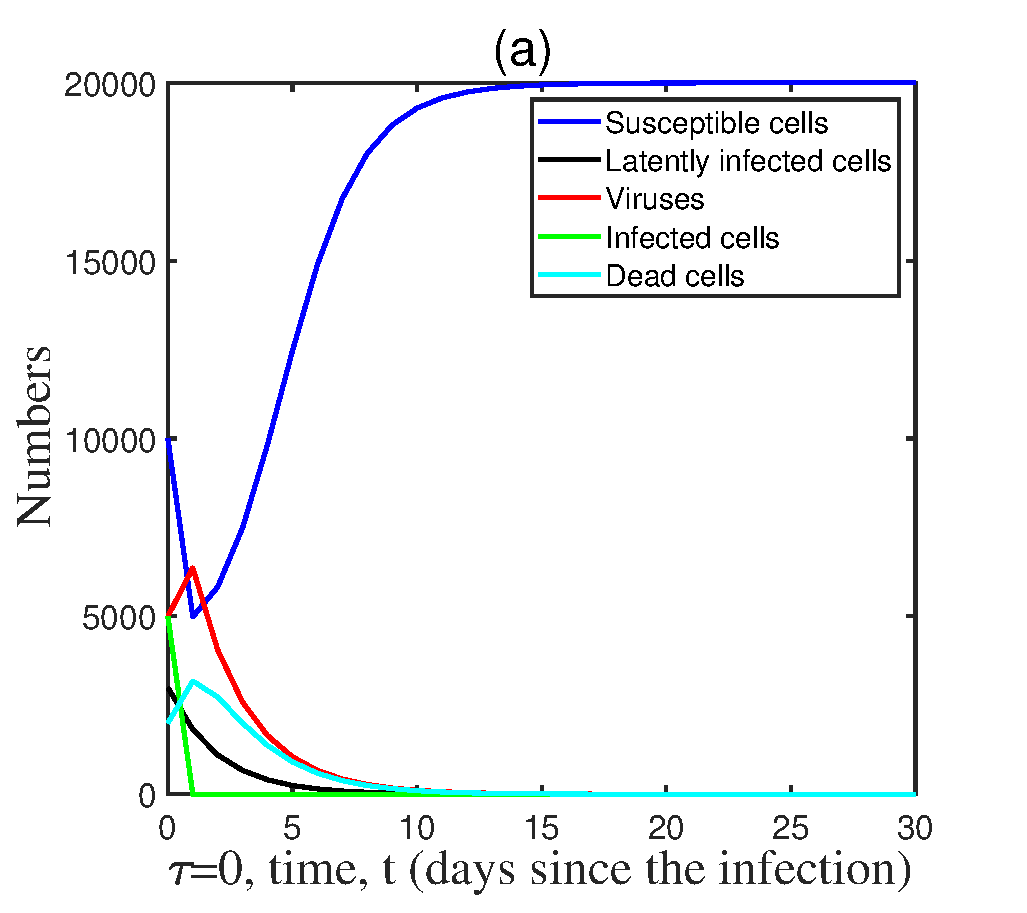
\includegraphics[height=0.16\textheight,width=0.3\textwidth]{G3.eps}
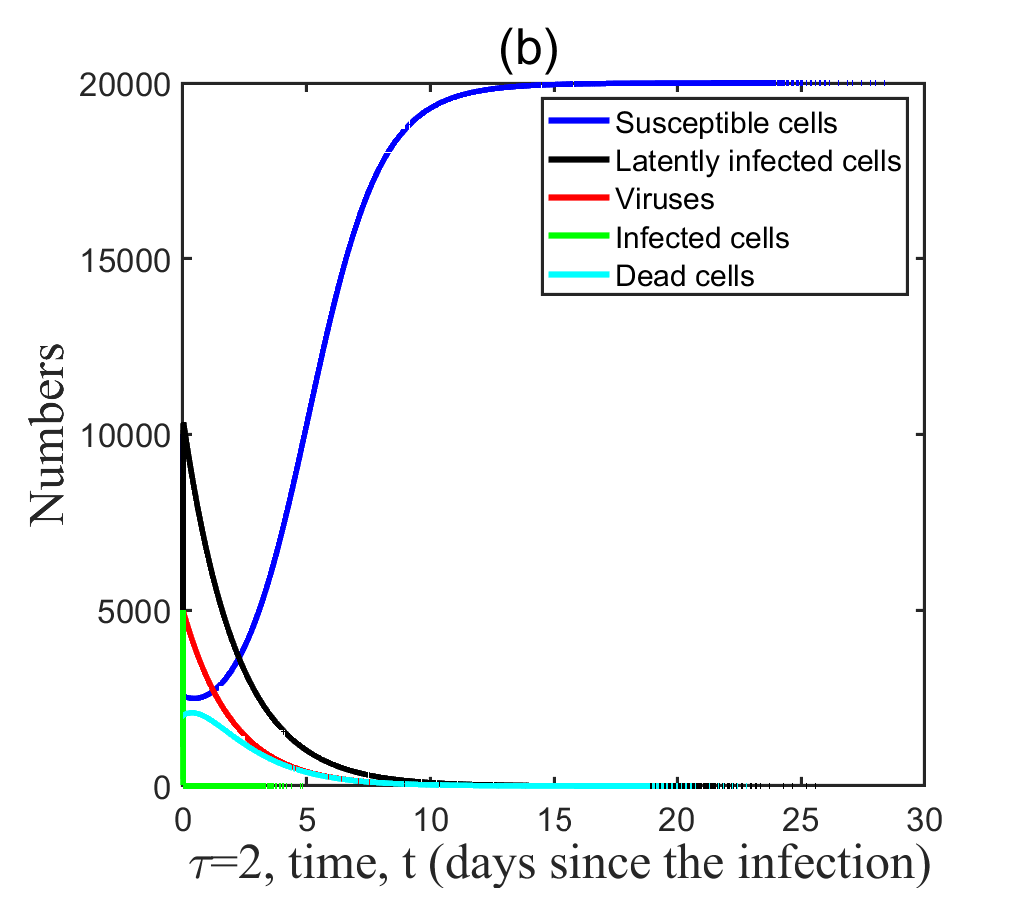
\includegraphics[height=0.16\textheight,width=0.3\textwidth]{G1.eps}
\vspace{3mm}
\caption{Time course plots of susceptible cells, infected cells, virus and dead cells corresponding to infection-free equilibrium when the basic regeneration number $R_0<1$. (a) The stability is predicted when $\tau=0$. (b) In the case of $\tau=2$.}
\label{Fig.2A}
\end{figure}

\begin{figure}[h!]
\centering
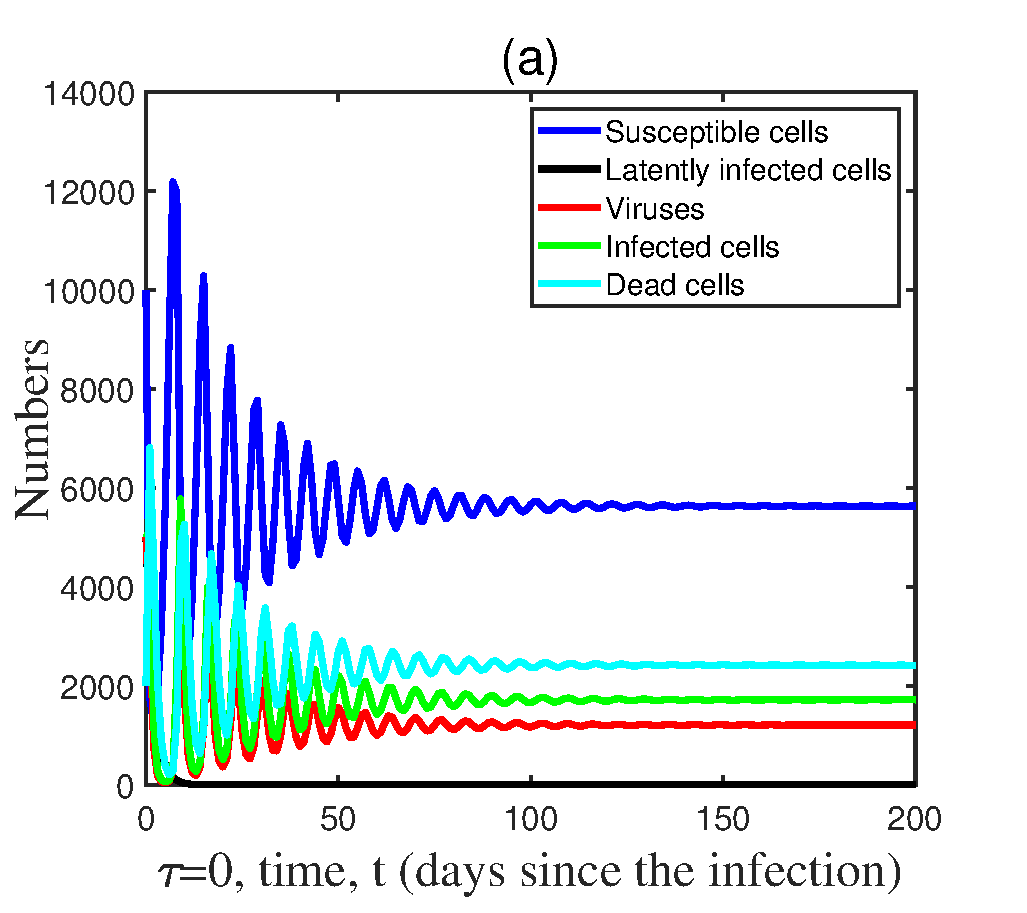
\includegraphics[height=0.16\textheight,width=0.3\textwidth]{H1.eps}
\includegraphics[height=0.16\textheight,width=0.3\textwidth]{H3.eps}\\
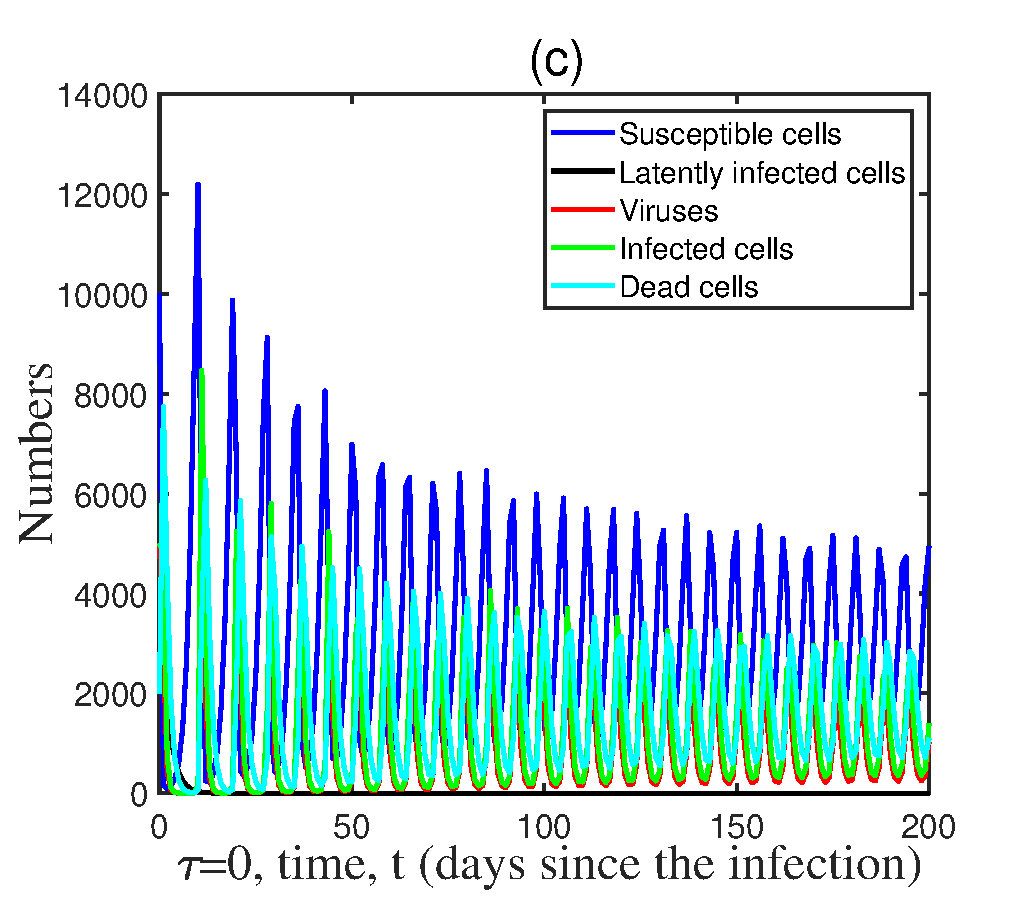
\includegraphics[height=0.16\textheight,width=0.3\textwidth]{H2.eps}
\includegraphics[height=0.16\textheight,width=0.3\textwidth]{H4.eps}
\vspace{3mm}
\caption{(a, c) Time course plots of susceptible cells, infected cells, virus and dead cells corresponding to infection-present equilibrium when $\tau=0$. (b, d) Phase diagrams of susceptible cells, infected cells and virus composition.}
\label{Fig.2}
\end{figure}

Next, we discuss the kinetic results of the time delay driven infection-present equilibrium point $E_1$. 
\jwmargin{Not sure what 'kinetic results' or 'time delay driven' means here.  Perhaps 'dependence of stability of infection-present equilibrium on time delay.}
Before examining the role of time delay, let us consider the case without time delay. Here, we use the following parameters: $p=30$ $day^{-1}$, $d_V=20$ $day^{-1}$, $s=0.8$ $day^{-1}$, $\Smax=20000$ $cells$ $mm^{-3}$, $d_I=2$ $day^{-1}$, $d_D=1$ $day^{-1}$, $\beta_1=0.00025$ $mm^{3}$ $cells^{-1}$ $day^{-1}$, $\beta_2=0.0002$ $mm^{3}$ $virus^{-1}$ $day^{-1}$, $\delta=0.005$ $day^{-1}$. We find that $\tau=0$, the infection-present equilibrium point is stable, as shown in \fig{Fig.2}(a)(b). When we change the infection rate to $\beta_1=0.475$, the infection-present equilibrium point is unstable, as shown in \fig{Fig.2}(c)(d). Under the set of parameters in \fig{Fig.2}(a)(b), we evaluate Conditions \hypothesis{2} in Section \ref{3.3} and obtain $h_1=662.028>0$, $h_2=2927.68>0$, and $h_3=22.9859>0$, thus \hypothesis{2} is satisfied. Under the set of parameters in \fig{Fig.2}(c)(d),  we obtain $h_1=474.05>0$, $h_2=-735.42<0$, and $h_3=31.9973>0$, thus \hypothesis{2} is not satisfied. Our simulations illustrate the results in Section \ref{3.3}.



Finally, time histories of susceptible cells, infected cells, virus, and dead cells approaching the equilibrium point of infection are plotted in \fig{Fig.20} under different time delays. When the time delay is small, the model is still stable, but becomes oscillatory when the time delay crosses the first critical value and undergoes a Hopf bifurcation, as shown in \fig{Fig.20}(a)(b). As the time delay increases across the second critical value, the model regains its stability and tends towards the infection-free equilibrium point, as shown in \fig{Fig.20}(c). In addition, the bifurcation diagram of the corresponding time delay is also given in \fig{Fig.3}. Also, according to equations (\ref{17}), (\ref{20}) and (\ref{21}) in Section \ref{3.3}, the corresponding graph of the function $\zeta_n(\tau)$ is drawn when $\omega(\tau)$ is a positive real root, which can be seen in \fig{Fig.3b}. These all illustrate that the model goes from stable to oscillating and back to a stable state as the time delay changes.
\begin{figure}[h!]
\centering
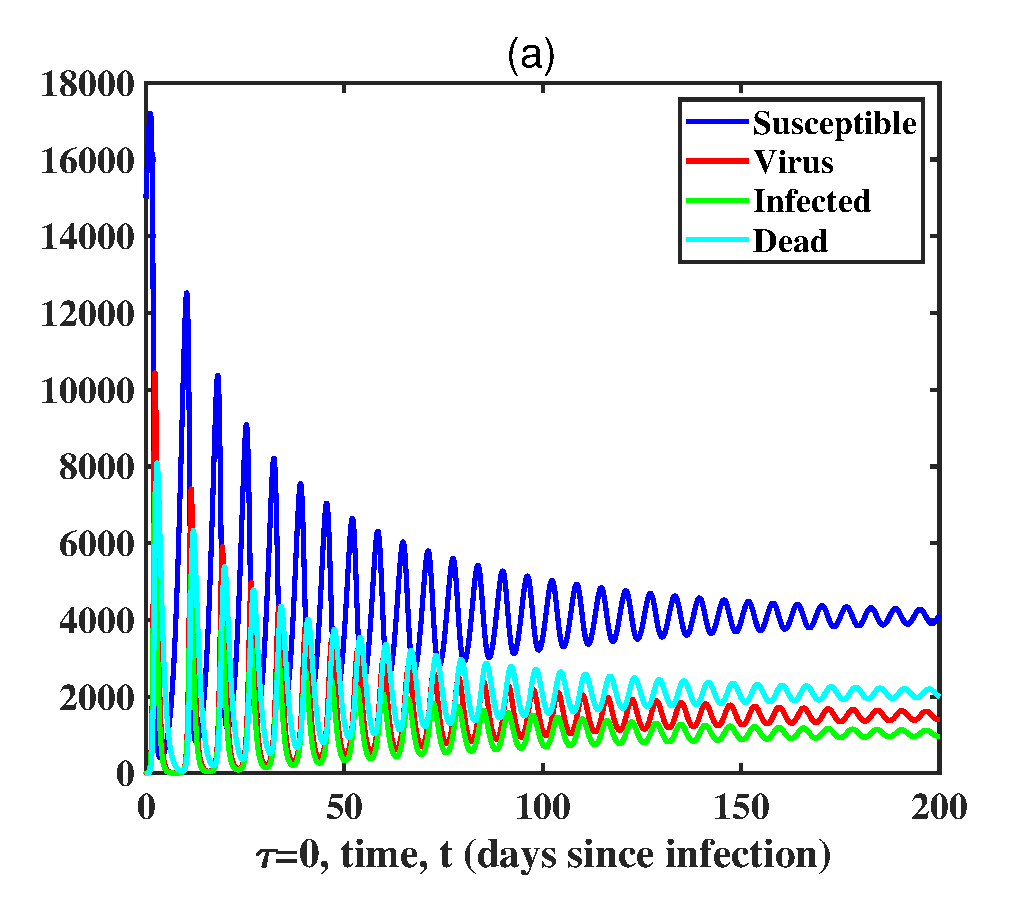
\includegraphics[height=0.16\textheight,width=0.3\textwidth]{I11.eps}
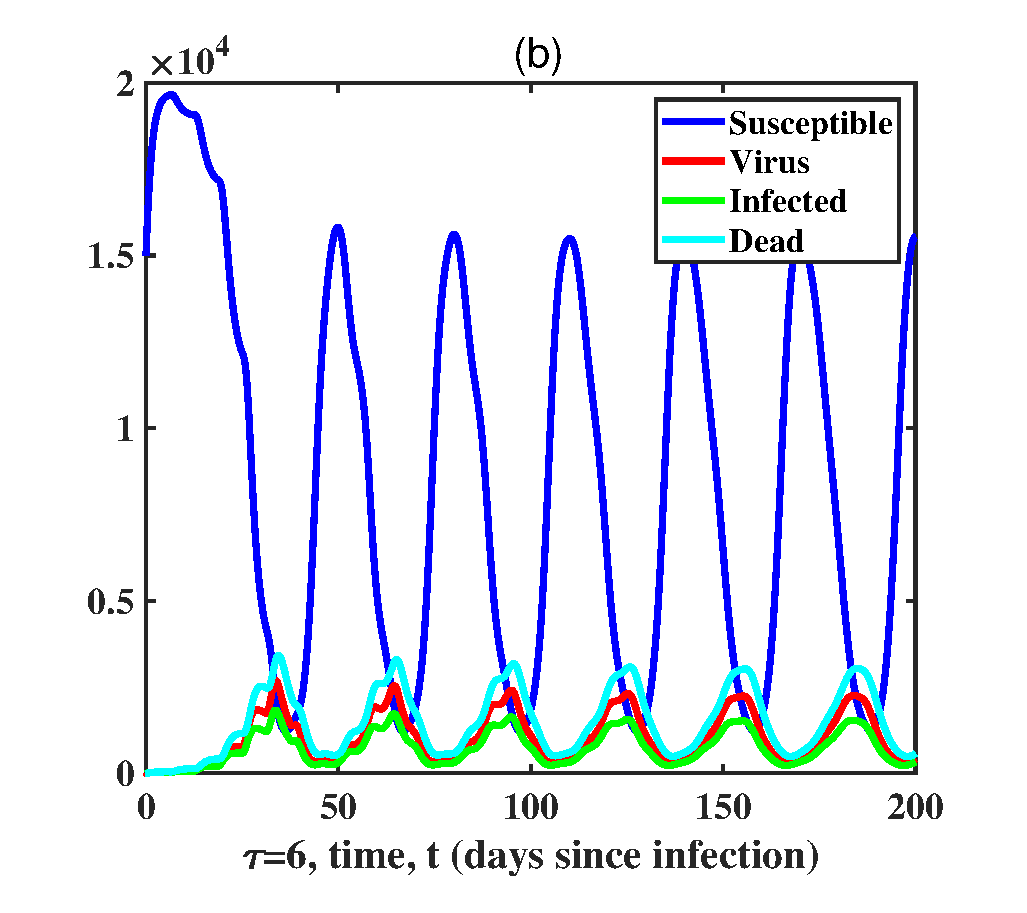
\includegraphics[height=0.16\textheight,width=0.3\textwidth]{I22.eps}
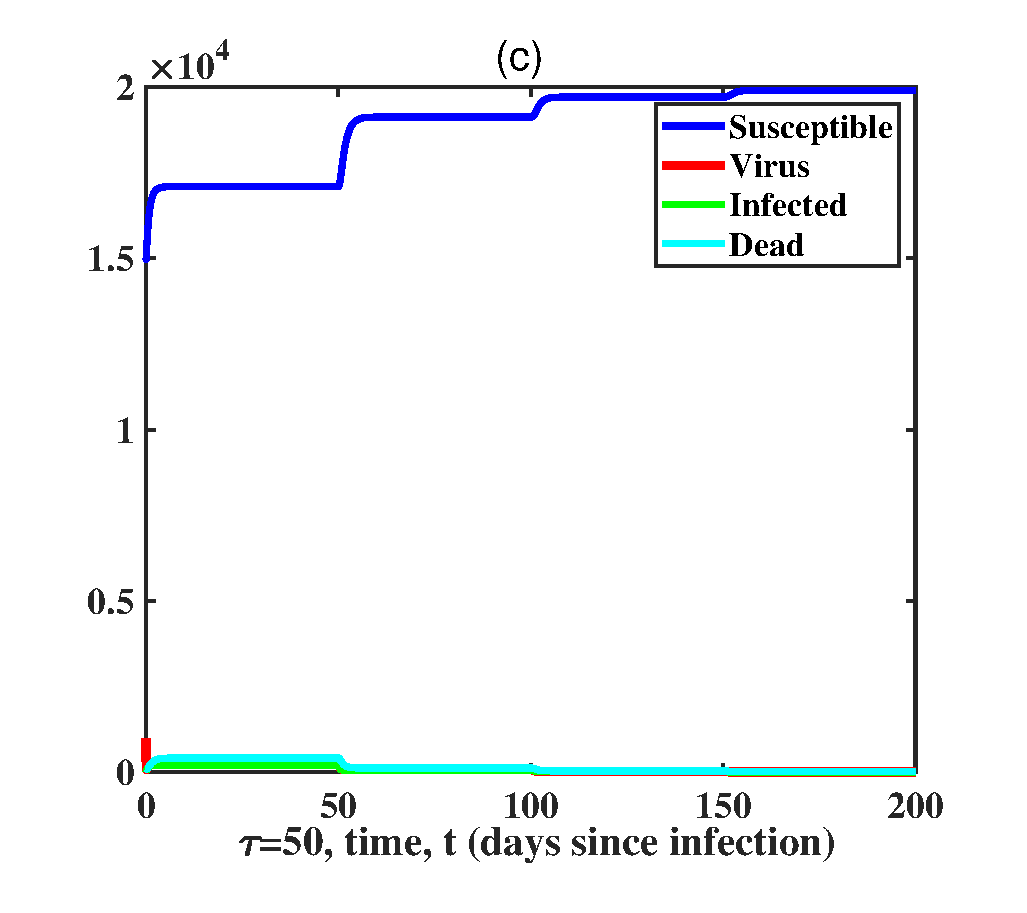
\includegraphics[height=0.16\textheight,width=0.3\textwidth]{I44.eps}
\vspace{3mm}
\caption{The dynamic effects of time-delay adjustment on SIVD model. (a) The positive equilibrium point is asymptotically stable when $\tau=0.04$. (b) When $\tau=6$, the positive equilibrium point is switched to the oscillatory state. (c) When $\tau=50$, the state of the equilibrium point of the SIVD model returns to a stable state again.}
\label{Fig.20}
\end{figure}



\begin{figure}[h!]
\centering
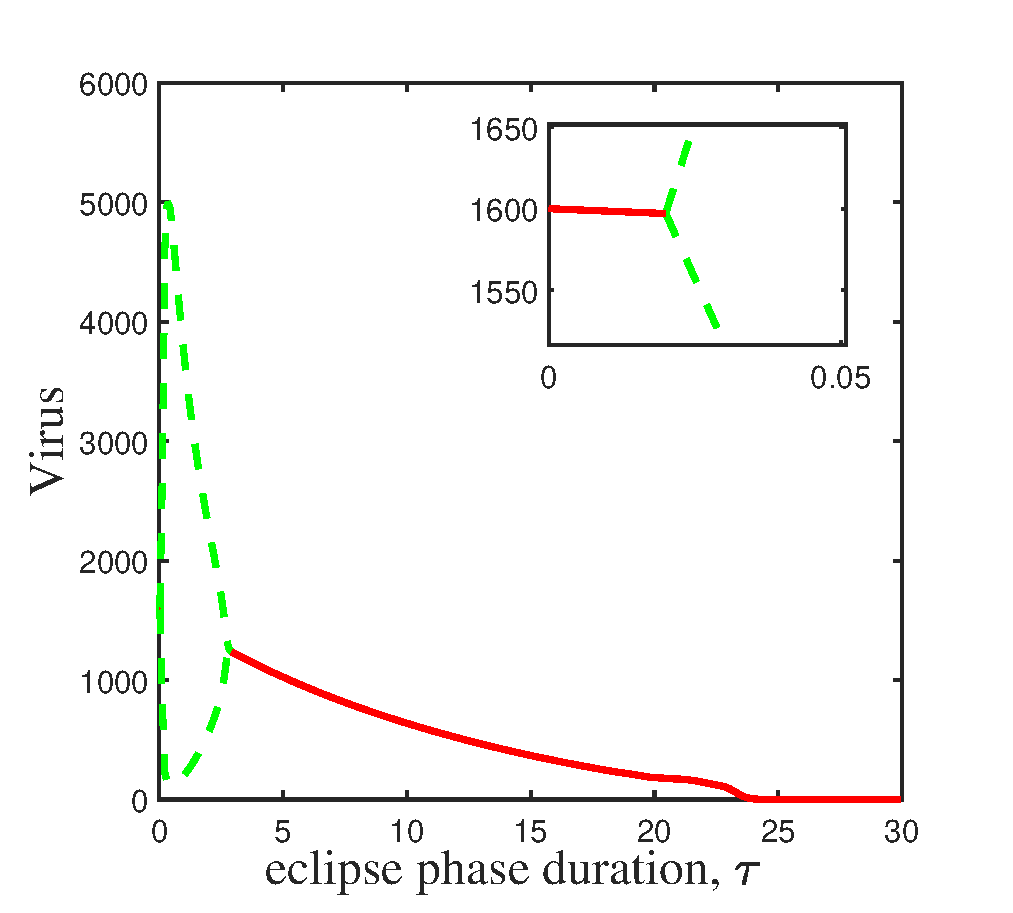
\includegraphics[height=0.2\textheight,width=0.35\textwidth]{J5.eps}
\vspace{3mm}
\caption{Bifurcation diagram of virus with increasing eclipse duration, $\tau$. The inset provides a clearer view of the left bifurcation point. The dashed curves indicate the minima and maxima along periodic orbits, light blue curves indicate a stable infection-present equilibrium.}
\label{Fig.3}
\end{figure}


\begin{figure}[h!]
\centering
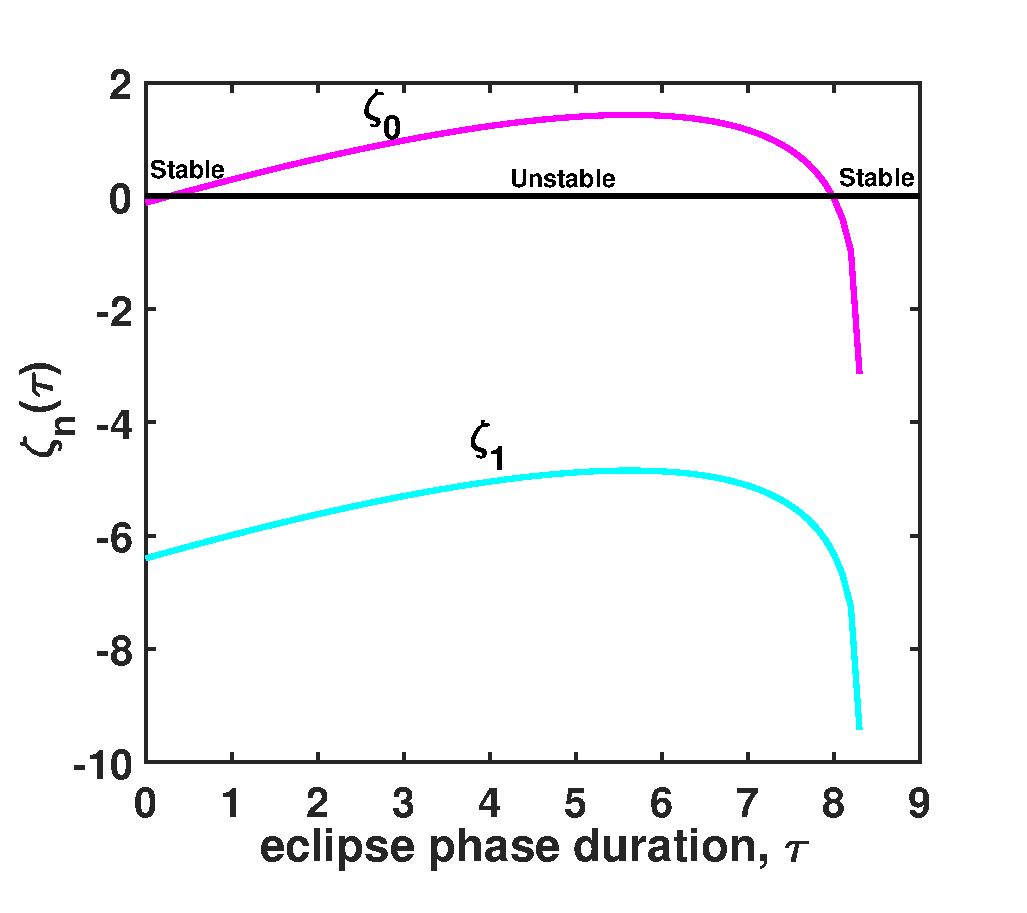
\includegraphics[height=0.2\textheight,width=0.35\textwidth]{F2.eps}
\vspace{3mm}
\caption{The graph corresponding to the function $\zeta_n(\tau)$. The magenta and cyan represent the curves of the functions $\zeta_0(\tau)$ and $\zeta_1(\tau)$, respectively.}
\label{Fig.3b}
\end{figure}
\subsection{Oscillatory behavior of the parameters-induced SIVD model}
In addition to the key role of time delay, the contribution of important parameters to the system oscillation behavior cannot be ignored. To this end,  in this section, we elaborate the contribution of the Virus infection rate $(\beta_1)$, the rate at which the virus enters susceptible cells $(\beta_2)$, the death rate of infected but not yet virus-producing cells $(\delta)$, and the rate actively-infected cells produce virus $(p)$ to the oscillatory mechanism of system dynamics. We mainly study the dynamical potential oscillatory behavior of the model through bifurcation analysis, as shown in Figures \ref{Fig.4} and \ref{Fig.6}. The red curve indicates a locally stable infection-present equilibrium, the black curve indicates an unstable infection-present equilibrium, and the green dotted line denotes the maximum and minimum along the limit cycle. The junction of red and black represents the Hopf bifurcation point.
\begin{figure}[h!]
\centering
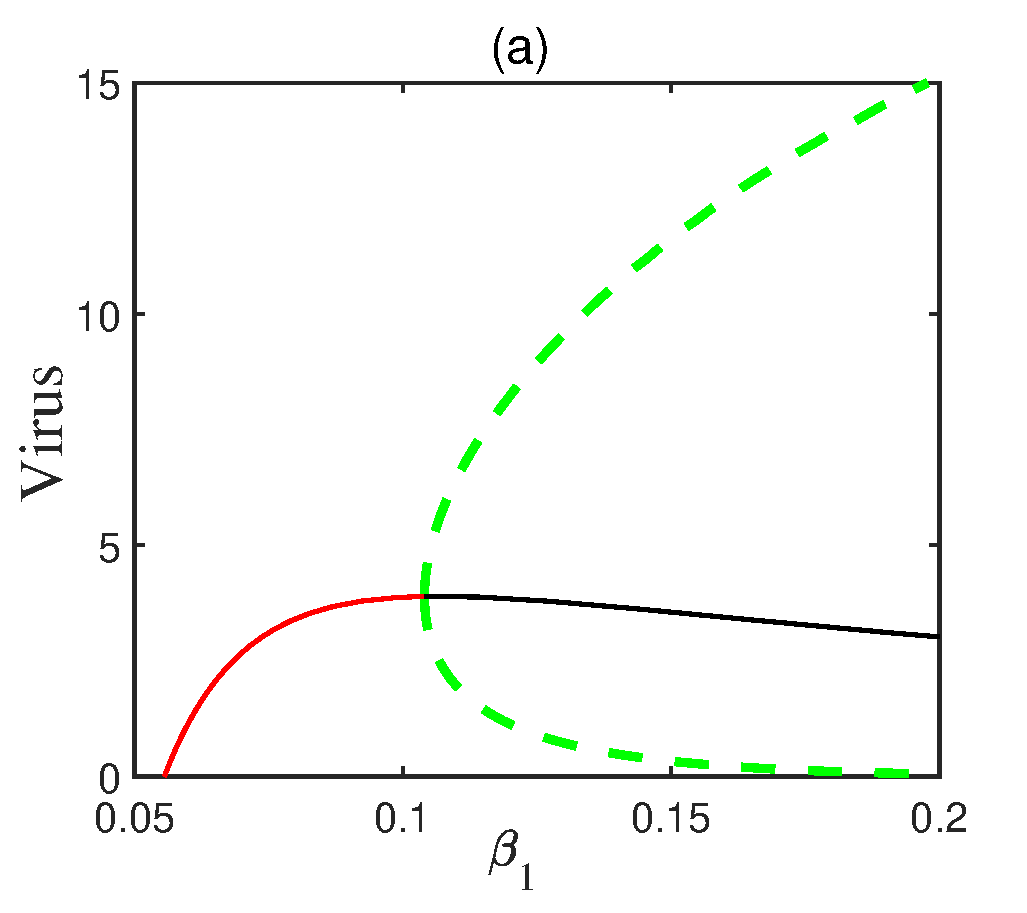
\includegraphics[height=0.20\textheight,width=0.35\textwidth]{A1.eps}
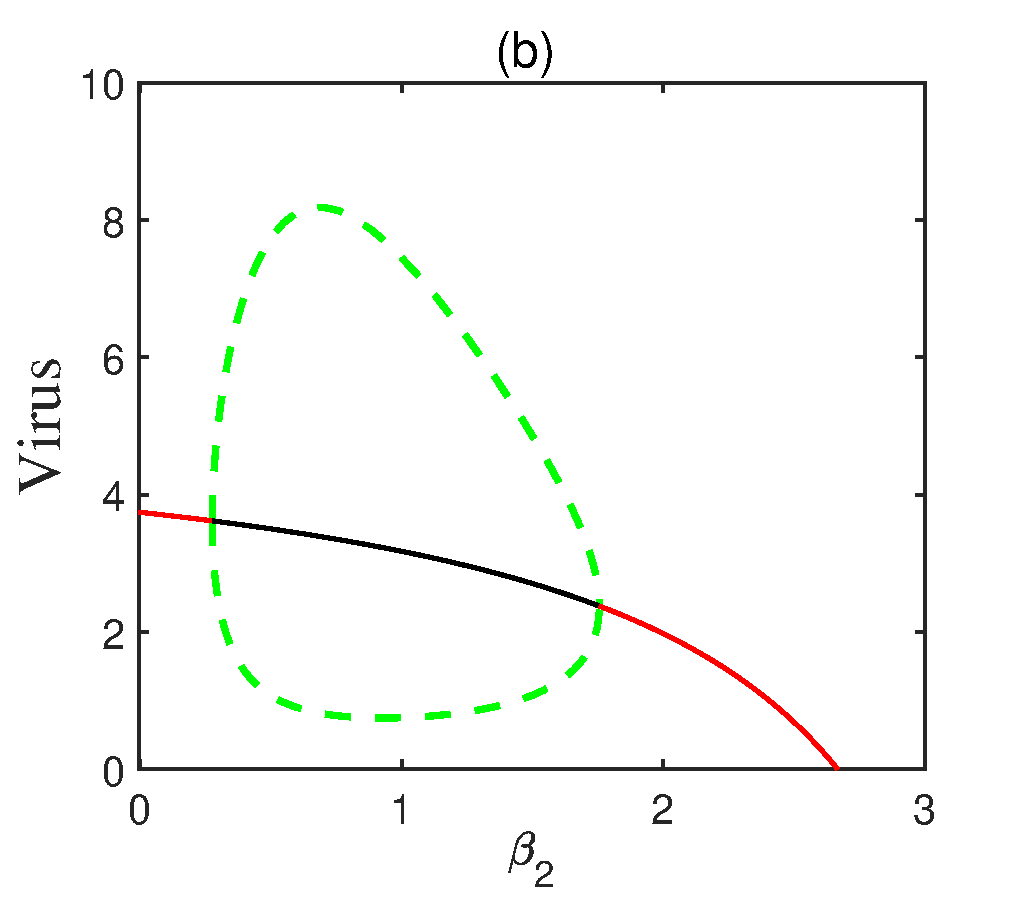
\includegraphics[height=0.20\textheight,width=0.35\textwidth]{A2.eps}
\vspace{3mm}
\caption{The bifurcation diagram level of virus infection model versus (a) virus infection rate ($\beta_1$) and (b) virus reduction rate ($\beta_2$). The junction of the red and black lines represents the Hopf bifurcation point. The red line represents the steady state, the black line represents the unstable state, and the green dots represent the limit cycle.}
\label{Fig.4}
\end{figure}

\begin{figure}[h!]
\centering
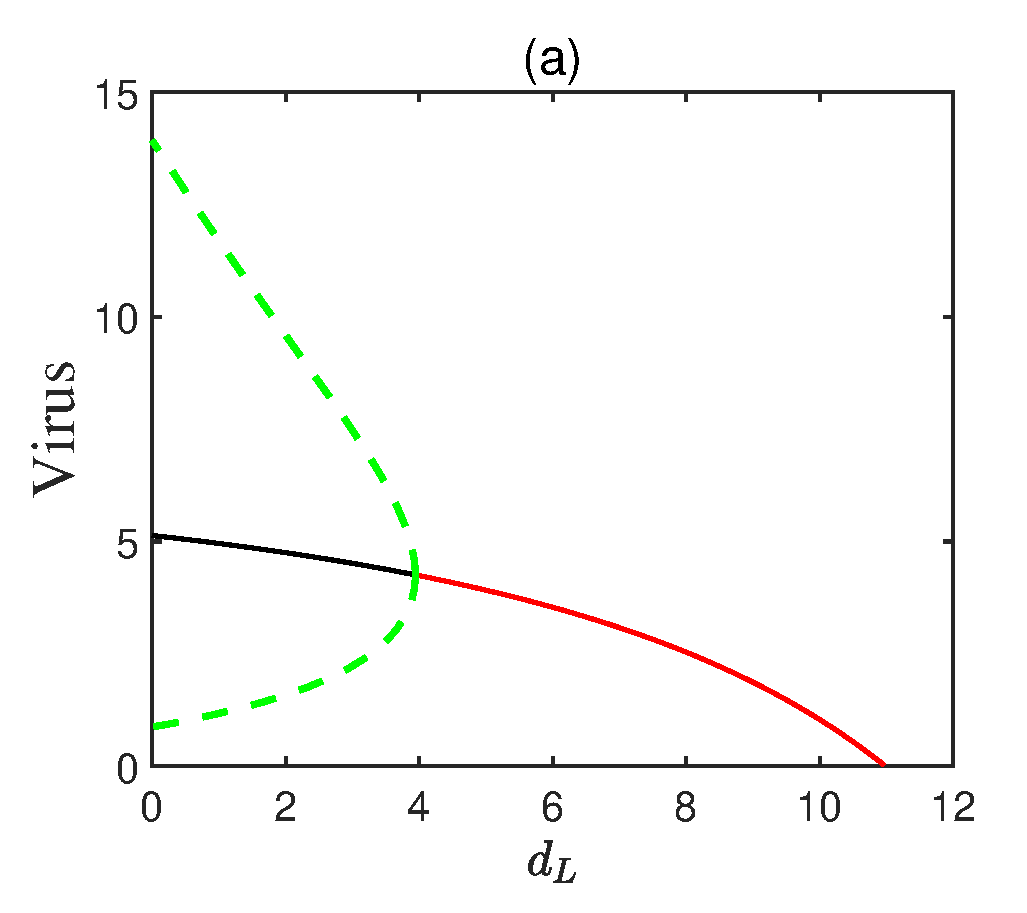
\includegraphics[height=0.20\textheight,width=0.35\textwidth]{A4.eps}
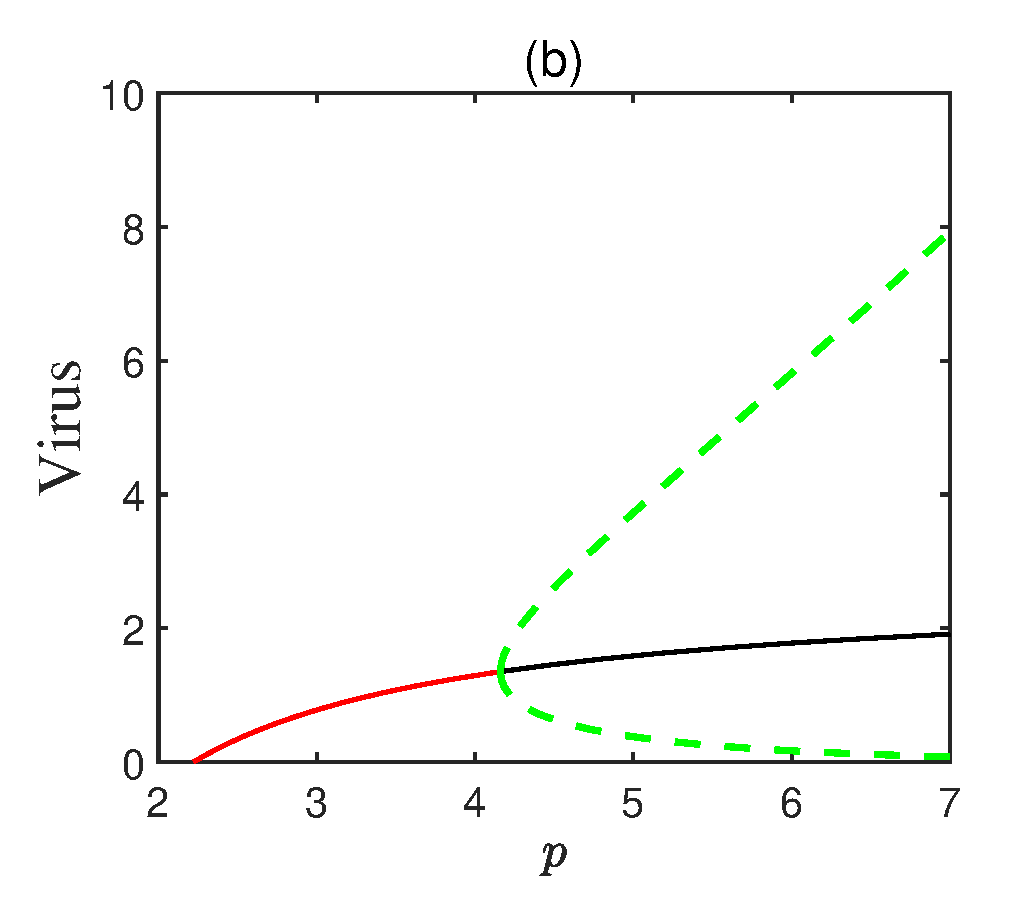
\includegraphics[height=0.20\textheight,width=0.35\textwidth]{A5.eps}
\vspace{3mm}
\caption{The bifurcation diagram level of virus infection model versus (a) mortality of cells infected but not yet producing virus ($\delta$), (b) rate of virus production by infected cells ($p$). The junction of the red and black lines represents the Hopf bifurcation point. The red line represents the steady state, the black line represents the unstable state, and the green dots represent the limit cycle.}
\label{Fig.6}
\end{figure}
From a biological point of view, reducing the rate at which host cells are infected $(\beta_1)$ is indisputably important for disease control. Therefore, to analyze how the oscillatory behavior of susceptible host cells is turned on or off in response to the infection rate, \fig{Fig.4}(a) is plotted. Specifically, the Hopf bifurcation point appears with the gradual increase of $(\beta_1)$, and susceptible host cells switch from a high steady state to a sustained oscillatory state. This result suggests that it is particularly important to use effective means to control the infection rate of host cells and maintain high steady state in host cells up to the maximum in susceptible cells. In this model, viral entry into host cells and thus viral reduction is also particularly important. Therefore, when the rate of virus entry into host cells is gradually increased, while the rate of host cell transformation into infected cells is small, the bifurcation diagram of host cells is shown in \fig{Fig.4}(b) is given. With the gradual increase of $\beta_2$, the level of susceptible cells initially maintained a low steady state, then experienced periodic oscillation after passing through the first Hopf bifurcation point, and finally the oscillation disappeared and returned to a high steady state after the second Hopf bifurcation point. From this, we know that with the increase of $\beta_2$, the susceptible cells increase. The reason is that with the increase of $\beta_2$, the virus gradually decreased, and thus the susceptible cells began to increase gradually. This can also be observed from the model. Next, a bifurcation diagram of Death rate for infected but not yet virus-producing cells ($\delta$) corresponding to the level of susceptible cells is presented in \fig{Fig.6} (a). As $\delta$ gradually increases, the level of susceptible cells undergoes a subcritical Hopf bifurcation. The level of susceptible cells transitions from a continuously oscillatory state to a high steady state. This suggests that increasing $\delta$ to high steady state of susceptible cells is more beneficial for disease control. Finally, the bifurcation diagram of susceptible cells level versus the The rate of infected cells produce virus ($p$) is plotted in Fig.\ref{Fig.6} (b). Initially with small $p$, susceptible cells maintain high stable state, and as $p$ continues to increase, the Hopf bifurcation emerges and undergoes a sustained oscillatory state. This suggests that controlling the rate at which infected cells produce virus and maintaining high stable state of susceptible cells is more effective in controlling viral infection.





\subsection{Combination control of time delay and other important parameters}

In this simulation section, Figs. \ref{Fig.8} are plotted to explore the dynamic behavior of the model with different parameters and delays. 
\fig{Fig.8}(a) shows two-parameter bifurcation diagrams of $\beta_1$ and $\beta_2$ at different time delays, and these different curves all represent Hopf bifurcation points. We observe that as the delay increases, the $\beta_1$ bifurcation point increases, the $\beta_2$ left bifurcation point increases and the right bifurcation point decreases. \fig{Fig.8}(b) shows the two-parameter bifurcation diagrams of $\beta_2$ and $p$ at different time delays. We find that as the delay increases, the $p$ bifurcation point increases, the $\beta_2$ left bifurcation point increases and the right bifurcation point decreases. \fig{Fig.8}(c) shows the two-parameter bifurcation diagrams of $\beta_1$ and $\delta$ at different time delays. We find that as the delay increases, the $\beta_1$ bifurcation point decreases and the $\delta$ bifurcation point increases. \fig{Fig.8}(d) shows the two-parameter bifurcation diagrams of $\delta$ and $\beta_2$ at different delays. We find that as the delay increases, the $\delta$ bifurcation point decreases, the $\beta_2$ left bifurcation point increases, and the right bifurcation point decreases. \fig{Fig.8}(e) shows the two-parameter bifurcation diagrams of $d_D$ and $\beta_2$ at different time delays. We can understand that when the time delay is small, when $\beta_2$=0.7 or so, there are three branch points in $d_D$ that are stable to oscillating to stable and oscillating again. However, when the time delay is larger, this situation disappears. In addition, when the delay increases, the left bifurcation point of $d_D$ is almost constant, and the right bifurcation point decreases. When $d_D$ is small, the left bifurcation point of $\beta_2$ is almost unchanged. When $d_D$ increases, the left bifurcation point increases and the right bifurcation point decreases. \fig{Fig.8}(f) shows the two-parameter bifurcation diagrams of $d_V$ and $d_D$ at different time delays. The bifurcation point of $d_V$ decreases with the increase of time delay, but the change is not obvious. When $d_V$ is small, there is a single bifurcation point in $d_D$, and when $d_V$ is larger, there are two bifurcation points in $d_D$.
%Finally, the sensitivity analysis of the time-delay bifurcation point to all parameters is given. It can be seen from \fig{Fig.9} that the most sensitive is $\beta_1$, followed by $p$, and the least sensitive to $\delta$.
\begin{figure}[h!]
\centering
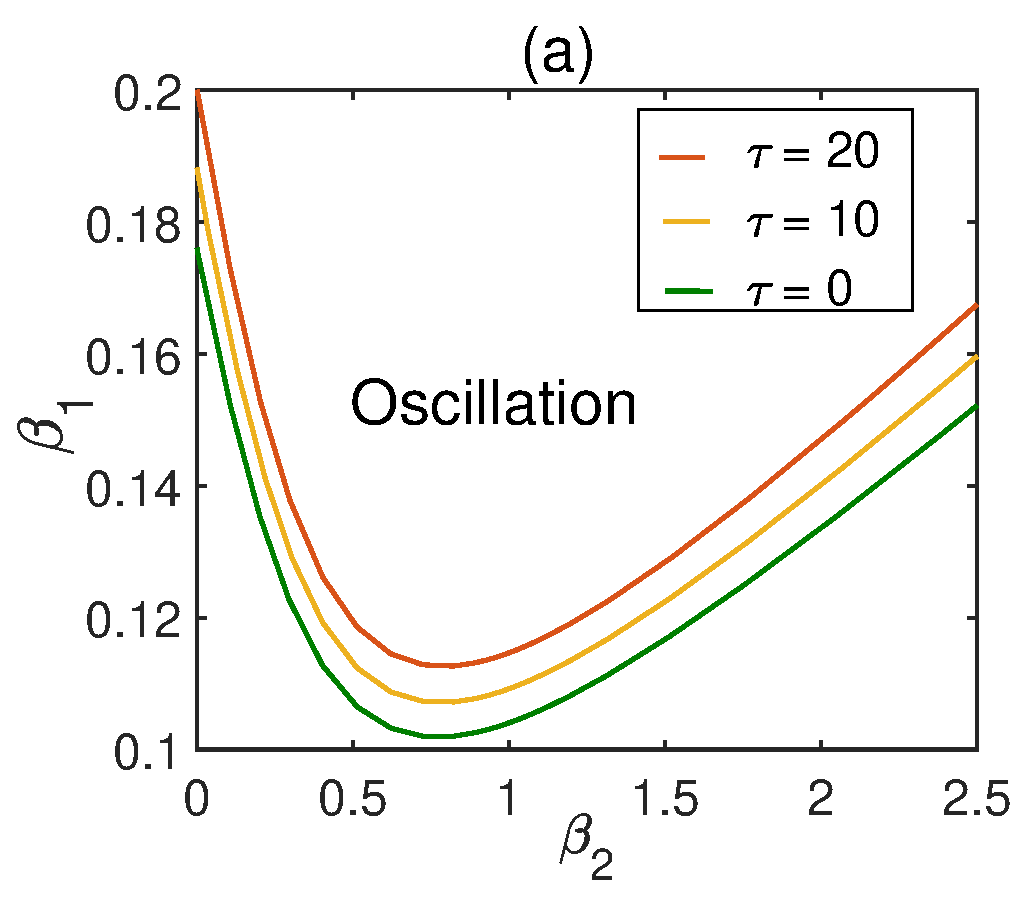
\includegraphics[height=0.15\textheight,width=0.29\textwidth]{A3.eps}
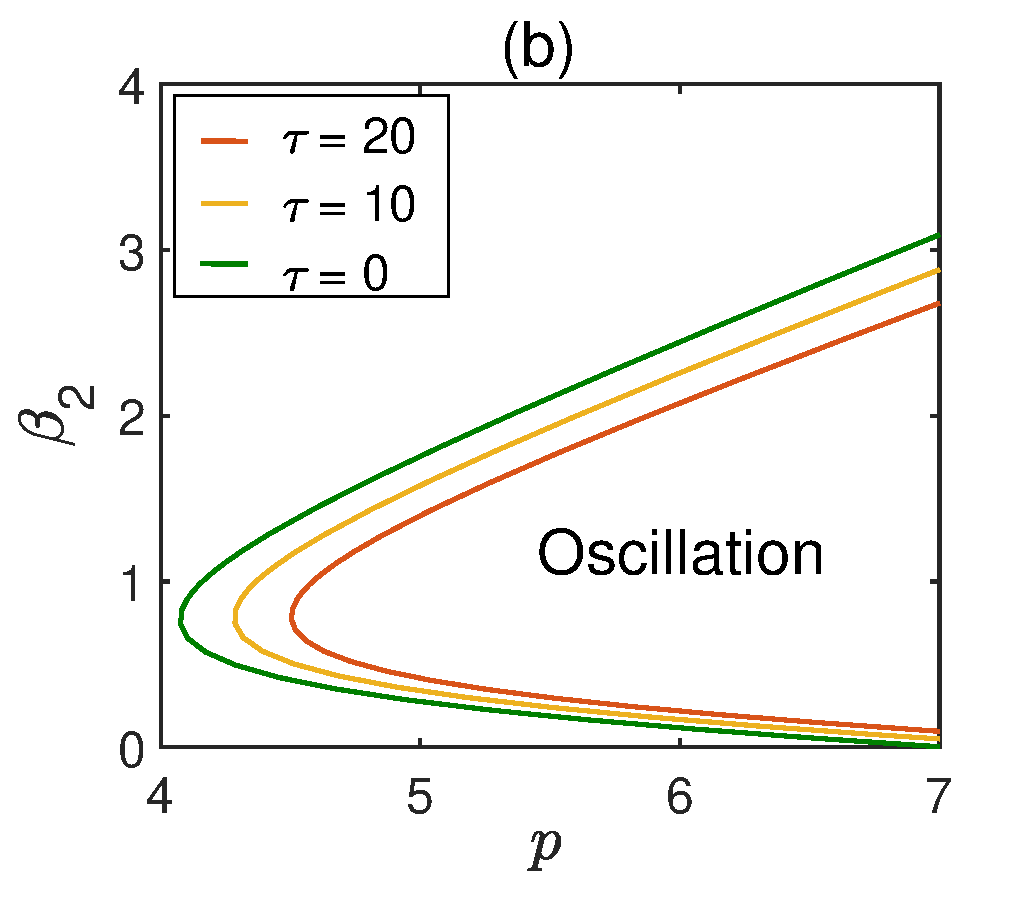
\includegraphics[height=0.15\textheight,width=0.29\textwidth]{A6.eps}
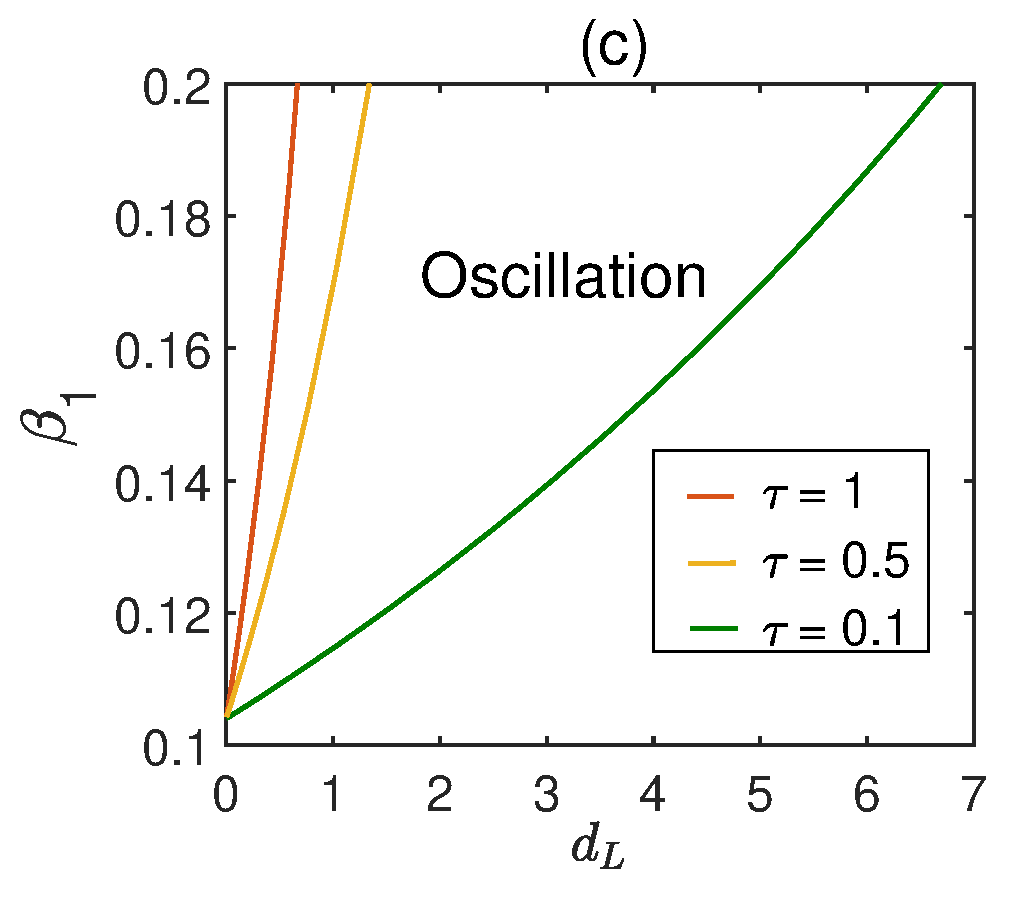
\includegraphics[height=0.15\textheight,width=0.29\textwidth]{A7.eps}
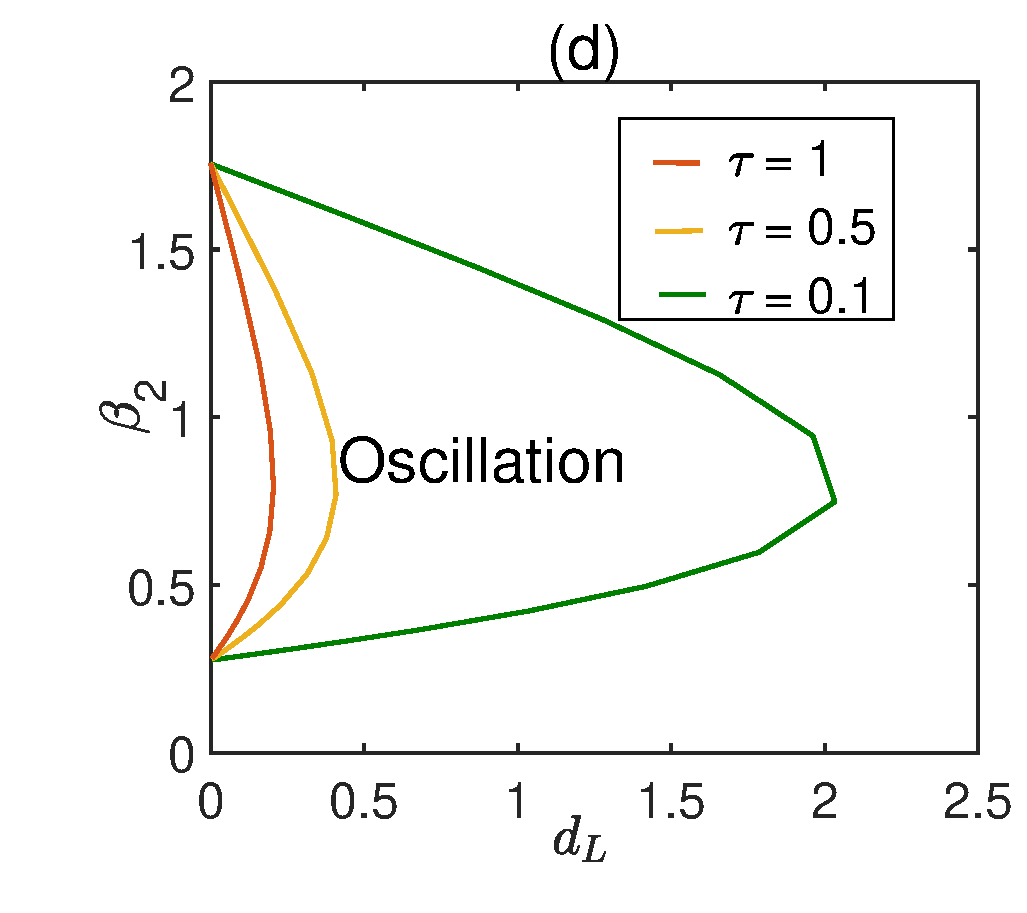
\includegraphics[height=0.15\textheight,width=0.29\textwidth]{A8.eps}
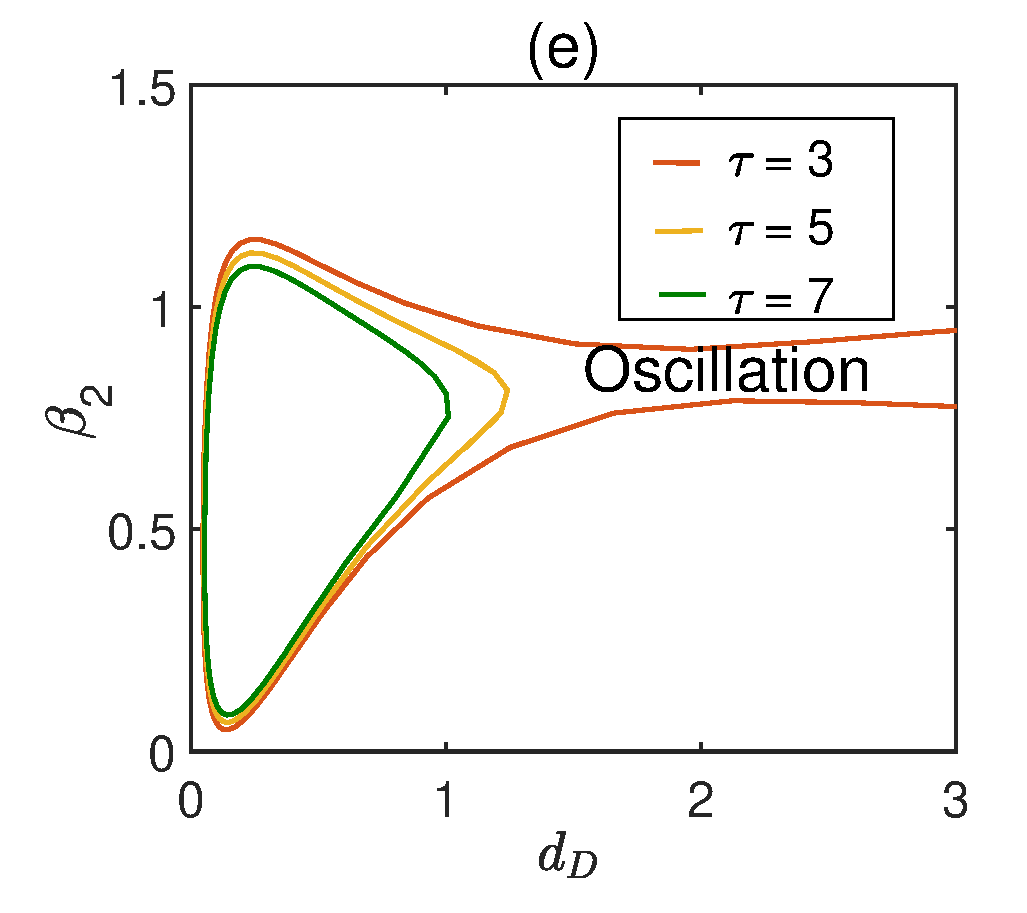
\includegraphics[height=0.15\textheight,width=0.29\textwidth]{A9.eps}
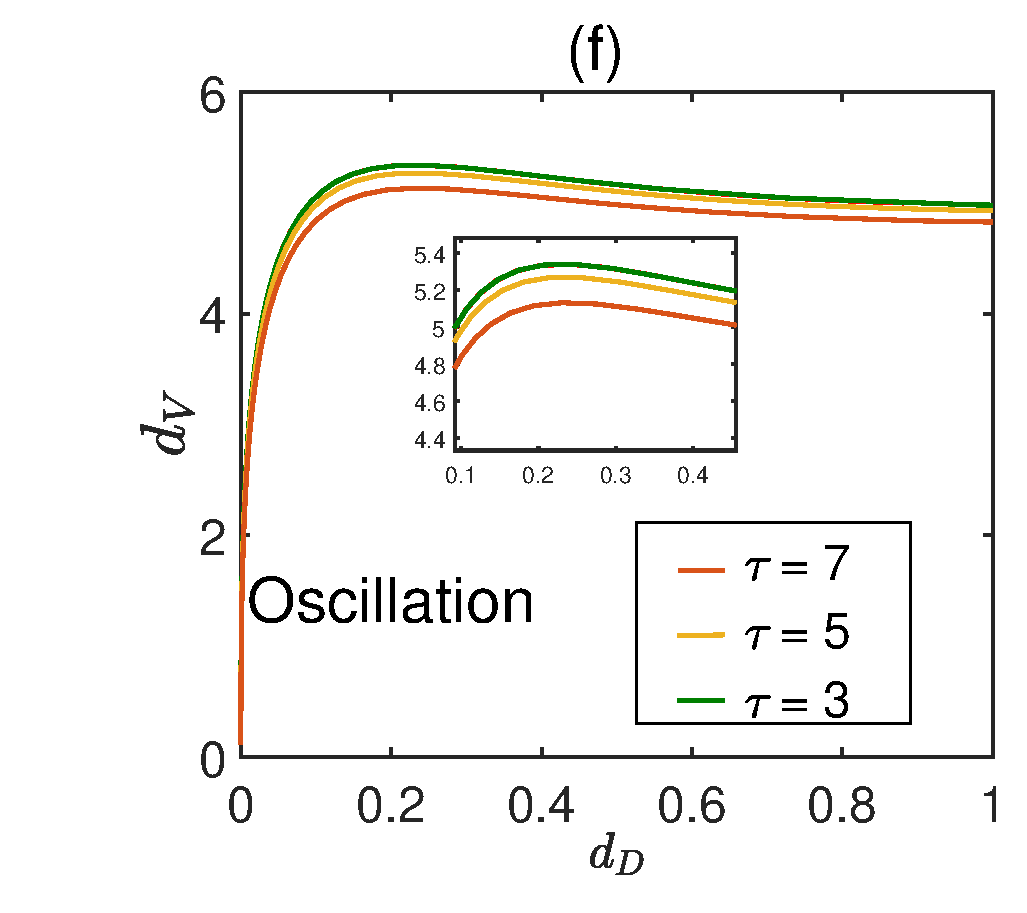
\includegraphics[height=0.15\textheight,width=0.29\textwidth]{A10.eps}
\vspace{3mm}
\caption{Two-parameter analysis between different important parameters in the case of corresponding different time delays.}
\label{Fig.8}
\end{figure}
%\begin{figure}[h!]
%\centering
%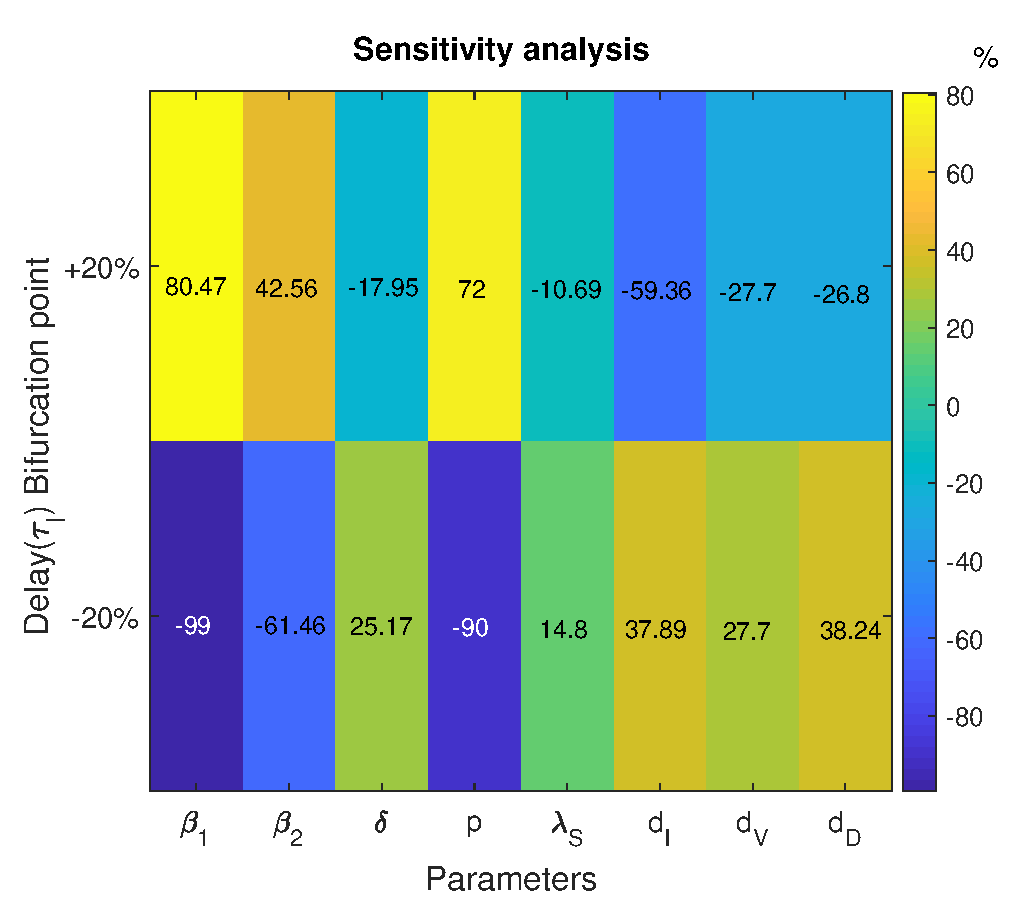
\includegraphics[height=0.25\textheight,width=0.45\textwidth]{E1.eps}
%\vspace{3mm}
%\caption{Sensitivity analysis plot of the delay bifurcation point to all parameters.}
%\label{Fig.9}
%\end{figure}

\section{Discussion} \label{sec5}
In this paper, we consider a relatively simple model of viral infection that incorporates an eclipse-time delay.  We provide both theoretical and computational analses of the model. First, we compute the basic reproduction number, $R_0$, and prove the global stability of the infection-free equilibrium for $R_0\leq 1$. Second, we prove the existence and examine the stability of the infection-present equilibrium for $R_0>1$: this equilibrium undergoes Hopf bifurcations, and we study their dependence on the eclipse-time delay. 
Our theoretical analysis show that the infection-free equilibrium point is stable when $R_0 < 1$, and unstable when $R_0 > 1$.
In the absence of time delay, the infection-present equilibrium point is stable under Assumption \hypothesis{2} and unstable otherwise. 
In the presence of delay, the delay, $\tau$, is considered as a bifurcation parameter.  As the delay increases across a threshold the infection-present equilibrium, $E_1$, undergoes a Hopf bifurcation, giving rise to oscillatory behaviour.
From the point of view of numerical simulation, our results show that firstly at $\tau=0$, when the assumed condition is satisfied, the infection equilibrium point is stable, otherwise it is unstable, which is consistent with the theoretical analysis. 
Second, we observe that as the delay increases, the system transitions from a stable state to an unstable state via the first Hopf bifurcation point, and then the delay continues to increase and the system regains its lost stability. In addition, the graph corresponding to the function $\zeta_n(\tau)$ is given. There are still two Hopf bifurcation points (see \fig{Fig.3}). Finally, we explore the impact of important parameters on the complex dynamics of the model,  including the infection rates $\beta_1$ and $\beta_2$, the mortality rate of eclipse-phase cells, $\delta$, the rate of virus production by infected cells, $p$, and the time delay, $\tau$. These are mainly reflected through single-parameter, two-parameter bifurcation diagrams, and three-parameter interaction.

There are still many open questions worthy of study on the basis of this research. For example, the important role of time delay in the kinetic model of immune infection and the cytokine kinetics involved in CoViD-19. From the theoretical analysis, the more complex dynamics generated by the delay, such as the global Hopf branch phenomenon \cite{shu2020complex,jiang2016global}, are more meaningful. In addition, from a biological point of view, the possible resistance effect of time delay against SARS-CoV-2 virus is also an interesting topic.



\section*{Acknowledgement}
LW and JW are supported by the Natural Sciences and Engineering Research Council of Canada.
\section*{Conflict of interest}
All authors declare no conflicts of interest in this paper.
%\section*{References}

\bibliography{mybibfile}

\end{document}
